\documentclass{article}

% preamble
\def\npart{III}
\def\nyear{2019}
\def\nterm{Lent}
\def\draft{Ongoing course}
\def\nlecturer{Professor B. L\"owe}
\def\ncourse{Topics in Set Theory}

\usepackage{imakeidx}
\usepackage{mathrsfs}
\usepackage{marginnote}
\usepackage{pbox}

\ifx \nauthor\undefined
  \def\nauthor{Bhavik Mehta}
\else
\fi

\author{Based on lectures by \nlecturer \\\small Notes taken by \nauthor}
\date{\nterm\ \nyear}
\title{Part \npart\ -- \ncourse}

\usepackage[utf8]{inputenc}
\usepackage{amsmath}
\usepackage{amsthm}
\usepackage{amssymb}
\usepackage{enumerate}
\usepackage{mathtools}
\usepackage{graphicx}
\usepackage[dvipsnames]{xcolor}
\usepackage{tikz}
\usepackage{wrapfig}
\usepackage{centernot}
\usepackage{float}
\usepackage{braket}
\usepackage[hypcap=true]{caption}
\usepackage{enumitem}
\usepackage[colorlinks=true, linkcolor=mblue]{hyperref}
\usepackage[nameinlink,noabbrev]{cleveref}
\usepackage{nameref}
\usepackage[margin=1.5in]{geometry}

% Theorems
\theoremstyle{definition}
\newtheorem*{aim}{Aim}
\newtheorem*{axiom}{Axiom}
\newtheorem*{claim}{Claim}
\newtheorem*{cor}{Corollary}
\newtheorem*{conjecture}{Conjecture}
\newtheorem*{defi}{Definition}
\newtheorem*{eg}{Example}
\newtheorem*{ex}{Exercise}
\newtheorem*{fact}{Fact}
\newtheorem*{law}{Law}
\newtheorem*{lemma}{Lemma}
\newtheorem*{notation}{Notation}
\newtheorem*{prop}{Proposition}
\newtheorem*{question}{Question}
\newtheorem*{rrule}{Rule}
\newtheorem*{thm}{Theorem}
\newtheorem*{assumption}{Assumption}

\newtheorem*{remark}{Remark}
\newtheorem*{warning}{Warning}
\newtheorem*{exercise}{Exercise}

% \newcommand{\nthmautorefname}{Theorem}

\newtheorem{nthm}{Theorem}[section]
\newtheorem{nlemma}[nthm]{Lemma}
\newtheorem{nprop}[nthm]{Proposition}
\newtheorem{ncor}[nthm]{Corollary}
\newtheorem{ndef}[nthm]{Definition}

% Special sets
\newcommand{\C}{\mathbb{C}}
\newcommand{\N}{\mathbb{N}}
\newcommand{\Q}{\mathbb{Q}}
\newcommand{\R}{\mathbb{R}}
\newcommand{\Z}{\mathbb{Z}}

\newcommand{\abs}[1]{\left\lvert #1\right\rvert}
\newcommand{\norm}[1]{\left\lVert #1\right\rVert}
\renewcommand{\vec}[1]{\boldsymbol{\mathbf{#1}}}

\let\Im\relax
\let\Re\relax

\DeclareMathOperator{\Im}{Im}
\DeclareMathOperator{\Re}{Re}
\DeclareMathOperator{\id}{id}

\definecolor{mblue}{rgb}{0., 0.05, 0.6}

\newtheorem*{observation}{Observation}

\usepackage{amssymb}% http://ctan.org/pkg/amssymb
\usepackage{pifont}% http://ctan.org/pkg/pifont
\usepackage{bbm}
\usetikzlibrary{cd}
\swapnumbers

\makeindex[intoc]

\renewcommand{\arraystretch}{1.3}

\newcommand{\named}[1]{\textbf{#1}\index{#1}}
\newcommand{\bonusnamed}[1]{\textbf{#1}\index{#1@*#1}}
\newcommand{\p}{\mathbb{P}}
\newcommand{\hf}{\textit{HF}}
\newcommand{\hc}{\textit{HC}}
\newcommand{\1}{\mathbbm{1}}
\newcommand{\cmark}{\ding{51}}%
\newcommand{\xmark}{\ding{55}}%
\DeclareMathOperator{\dom}{dom}
\DeclareMathOperator{\ran}{ran}
\DeclareMathOperator{\rk}{rk}
\DeclareMathOperator{\cons}{Cons}
\DeclareMathOperator{\tcl}{tcl}
\DeclareMathOperator{\Diag}{Diag}
\DeclareMathOperator{\Proj}{Proj}
\DeclareMathOperator{\Def}{Def}
\DeclareMathOperator{\name}{Name}
\DeclareMathOperator{\Fn}{Fn}
\DeclareMathOperator{\val}{val}
\newcommand{\zfc}{\textsf{ZFC}}

\setcounter{section}{-1}

\let\oldmodels\models
\let\models\vDash
\let\nModels\nvDash
\let\forces\Vdash

\tikzset{dot/.style={inner sep=1pt, fill=black, circle}}

% and here we go!
\begin{document}
\maketitle

\tableofcontents

\clearpage
\section{Introduction}
\newlec
The main `topic in set theory' covered in this course will be one of the most important: solving the Continuum Problem.
A priori, set theory does not seem intrinsically related to logic, but the continuum hypothesis showed that logic was a very important tool in set theory.
In contrast to many other disciplines of mathematics, in set theory we typically try to prove things are \emph{impossible}, rather than showing what is possible.

The second international congress of mathematicians in 1900 was in Paris, where Hilbert spoke. At that time, Hilbert was a `universal' mathematician, and had worked in every major field of mathematics. He gave a list of problems for the century, the 23 Hilbert Problems. The first on this list was the Continuum Problem.

\subsection{Continuum Hypothesis}\index{Continuum hypothesis}\hypertarget{def:ch}
Here is Hilbert's formulation of the Continuum hypothesis (CH):
Every set of infinitely many real numbers is either equinumerous with the set of natural numbers or the set of real numbers.
More formally, we might write
\begin{equation*}
  \forall X \subseteq \mathbb{R}, (X \text{ is infinite} \Rightarrow X \sim \mathbb{N} \text{ or } X \sim \mathbb{R})
\end{equation*}

In more modern terms, we write this as the claim $2^{\aleph_0} = \aleph_1$.
These two statements are equivalent (in \textsf{ZFC}).

Assume that $2^{\aleph_0} > \aleph_1$, in particular $2^{\aleph_0} \geq \aleph_2$. Since $2^{\aleph_0} \sim \mathbb{R}$, we get an injection $i: \aleph_2 \to \mathbb{R}$.
Consider $X \coloneqq i[\aleph_1] \subseteq \mathbb{R}$. Clearly, $i|_{\aleph_1}$ is a bijection between $\aleph_1$ and $X$, so $X \sim \aleph_1$.
But $\aleph_1 \nsim \mathbb{N}$ and $\aleph_1 \nsim \mathbb{R}$.
Thus $X$ refutes CH (in its earlier formulation).
So: $2^{\aleph_0} \neq \aleph_1 \implies \neg \text{CH}$.

If $2^{\aleph_0} = \aleph_1$.
Let $X \subseteq \mathbb{R}$. Consider $b: 2^{\aleph_0} \to \mathbb{R}$ a bijection. If $X$ is infinite, then $b^{-1}[X] \subseteq 2^{\aleph_0}$.
Thus the cardinality of $X$ is either $\aleph_0$, i.e.\ $X \sim \mathbb{N}$ or $\aleph_1$, i.e.\ $X \sim \mathbb{R}$.
So, $2^{\aleph_0} = \aleph_1 \implies \text{CH}$.

\subsection{History of CH}
\begin{itemize}[label=--]
  \item 1938, G\"odel: \textsf{ZFC} does not prove $\neg$\hyperlink{def:ch}{CH}.
  \item 1963, Cohen: \textsf{ZFC} does not prove CH.
\end{itemize}
G\"odel's proof used the technique of inner models; Cohen's proof used forcing, sometimes referred to as outer models.

G\"odel's Completeness Theorem:
\begin{equation*}
  \text{Cons}(T) \iff \exists(M, E) (M, E) \models T
\end{equation*}
From this, we might guess that G\"odel's and Cohen's proof will show there is a model of \textsf{ZFC} + CH, and a model of \textsf{ZFC} + $\neg$CH, but by the incompleteness phenomenon, we cannot prove there is a model of \textsf{ZFC}!
So, we are not going to be able to prove Cons(\textsf{ZFC}+CH), but instead
\begin{equation*}
  \text{Cons(\textsf{ZFC})} \rightarrow \text{Cons(\textsf{ZFC}+CH)}
\end{equation*}
Or, equivalently,
\begin{equation*}
  \text{if } M \models \text{\textsf{ZFC}, then there is } N \models \text{\textsf{ZFC} + CH}.
\end{equation*}

\clearpage
\section{Model theory of set theory}
Let's assume for a moment that
\begin{equation*}
  (M,\in) \models \text{\textsf{ZFC}}.
\end{equation*}
We refer to the canonical objects in $M$ by the usual symbols, e.g., $0,1,2,3,4,\dotsc, \omega, \omega+1, \dotsc$

What would an ``inner model'' be?
Take $A \subseteq M$, and consider $(A, \in)$. This is a substructure of $(M, \in)$.
Note: the language of set theory has no function or constant symbols. But we write down
\begin{equation*}
  X = \emptyset,\ X = \{Y\},\ X = \{Y,Z\},\ X = \bigcup Z,\ X = \mathcal{P}(Z)
\end{equation*}
which appear to use function or constant symbols. These are technically not part of the language of set theory; they are abbreviations:
\begin{align*}
  X &= \emptyset & &\text{ abbreviates } & &\forall w\; (\neg w \in X) \\
  X &= \{Y\} & & \text{ abbreviates } & &\forall w\; (w \in X \leftrightarrow w = Y) \\
  X &\subseteq Y & & \text{ abbreviates } & &\forall w\; (w \in X \rightarrow w \in Y)
\end{align*}
and so on.

\begin{defi}\hypertarget{def:abso}
  If $\varphi$ is a formula in $n$ free variables. We say
  \begin{enumerate}[label=(\arabic*)]
    \item $\varphi$ is \named{upwards absolute}\index{absolute!upwards-} between $A$ and $M$ if
      \begin{equation*}
        \text{for all } a_1, \dotsc, a_n \in A,\quad (A,\in) \models \varphi(a_1, \dotsc, a_n) \implies (M, \in) \models \varphi(a_1, \dotsc, a_n)
      \end{equation*}
    \item $\varphi$ is \named{downwards absolute}\index{absolute!downwards-} between $A$ and $M$ if
      \begin{equation*}
        \text{for all } a_1, \dotsc, a_n \in A,\quad (M,\in) \models \varphi(a_1, \dotsc, a_n) \implies (A, \in) \models \varphi(a_1, \dotsc, a_n)
      \end{equation*}
    \item $\varphi$ is \named{absolute} between $A$ and $M$ if it is upwards absolute and downwards absolute.
  \end{enumerate}
\end{defi}

\begin{defi}
  We\index{quantifier-free} say that a formula is \hypertarget{def:sig1}$\Sigma_1$ if it is of the form
  \begin{equation*}
    \exists x_1 \dotsc \exists x_n\ \varphi(x_1, \dotsc, x_n) \text{ where } \varphi \text{ is quantifier-free}
  \end{equation*}
  or \hypertarget{def:pi1}{$\Pi_1$} if it is of the form
  \begin{equation*}
    \forall x_1 \dotsc \forall x_n\ \varphi(x_1, \dotsc, x_n) \text{ where } \varphi \text{ is quantifier-free}.
  \end{equation*}
\end{defi}

\begin{remark}
  \leavevmode
  \begin{enumerate}[label=(\alph*)]
    \item If $\varphi$ is quantifier-free, then $\varphi$ is \hyperlink{def:abso}{absolute} between $A$ and $M$.
    \item If $\varphi$ is \hyperlink{def:pi1}{$\Pi_1$}, then it's \hyperlink{def:abso}{downward absolute}
    \item If $\varphi$ is \hyperlink{def:sig1}{$\Sigma_1$}, then it's \hyperlink{def:abso}{upward absolute}
  \end{enumerate}
\end{remark}

\newlec
Under our assumption that $(M,\in) \models \text{\textsf{ZFC}}$, which subsets $A \subseteq M$ give a model of \textsf{ZFC}?
Using standard model theory, we observed that if $\varphi$ is quantifier-free, then $\varphi$ is \hyperlink{def:abso}{absolute} between $(A,\in)$ and $(M,\in)$, but hardly anything is quantifier-free:
\begin{equation*}
  \hypertarget{def:phi0}x = \emptyset \iff \forall w\ (w \notin x) \eqqcolon \Phi_0(x)
\end{equation*}

For instance, suppose $A \coloneqq M \setminus \{1\}$ (recall $0,1,2,\dotsc$ refer to the ordinals in $M$).
In $A$, we have $0,2,\{1\}$. Clearly $(M,\in) \models \Phi_0(0)$.
$\Phi_0(x)$ is a \hyperlink{def:pi1}{$\Pi_1$} formula, so by $\Pi_1$-\hyperlink{def:abso}{downwards absoluteness}, $(A,\in) \models \Phi_0(0)$.

In reality, $2 = \{0,1\}$, but $1$ is not in $A$, so informally in $A$, the object $2$ has only one element.
Similarly, in $A$, $\{1\}$ has no elements, since $1$ is missing from $A$. Thus
\begin{equation*}
  (A,\in) \models \Phi_0(\{1\}).
\end{equation*}
Clearly $(M,\in) \nModels \Phi_0(\{1\})$, so $\Phi_0$ is not \hyperlink{def:abso}{absolute} between $A$ and $M$.
As a corollary, we get $(A,\in) \nModels$ Extensionality, since $0$ and $\{1\}$ have the same elements in $A$, but are not equal.

(Remark: We could go on, defining formulas $\Phi_1(x), \Phi_2(x)$ etc.\ to analyse which of the elements correspond to the natural numbers in $A$.)

\begin{defi}\hypertarget{def:transitive}
  We call $A$ \named{transitive} in $M$, if for all $a \in A$ and $x \in M$ such that $(M,\in) \models x \in a$, we have $x \in A$.
\end{defi}
\begin{prop}
  If $A$ is \hyperlink{def:transitive}{transitive}, then \hyperlink{def:phi0}{$\Phi_0$} is \hyperlink{def:abso}{absolute} between $A$ and $M$.
\end{prop}
\begin{proof}
  Since \hyperlink{def:phi0}{$\Phi_0$} is \hyperlink{def:pi1}{$\Pi_1$}, we only need to show \hyperlink{def:abso}{upwards absoluteness}.
  Suppose $a \in A$, such that $(A,\in) \models \Phi_0(a)$.
  Suppose $a \neq 0$. Thus there is some $x \in a$. By \hyperlink{def:transitive}{transitivity}, $x \in A$.
  So $(A,\in) \models x \in a$ and so $(A,\in) \nModels \Phi_0(a)$, contradiction.
\end{proof}
(Similarly, if $\Phi_n$ is the formula describing the natural number $n$, and there is $a \in A$ such that $(A,\in) \models \Phi_n(a)$ and $A$ is \hyperlink{def:transitive}{transitive}, then $a = n$.)
\begin{prop}
  If $A$ is \hyperlink{def:transitive}{transitive} in $M$, then
  \begin{equation*}
    (A,\in) \models \textsf{Ext}.
  \end{equation*}
\end{prop}
\begin{proof}
  Take $a,b \in A$ with $a \neq b$.
  By Extensionality in $(M,\in)$, find without loss of generality some $c \in a \setminus b$.
  Since $c \in a \in A$, by \hyperlink{def:transitive}{transitivity}, $c \in A$.
  Thus
  \begin{align*}
    (A,\in) &\models c \in a \\
    (A,\in) &\models c \notin b,
  \end{align*}
  so $a$ and $b$ do not satisfy the assumptions of Extensionality.
\end{proof}

Consider now $A \coloneqq \omega + 2 \subseteq M$, the ordinal consisting of $\{0,1,2,\dotsc, \omega, \omega+1\}$.
This is a transitive subset of $M$ (since it's an ordinal).
So
\begin{equation*}
  (A,\in) \models \textsf{Ext}.
\end{equation*}
Consider the formula $x = \mathcal{P}(y)$, which we can informally define as $x = \{z \mid z \subseteq y\}$, but this is not good enough. More properly, we try
\begin{equation*}
  x = \mathcal{P}(y) \iff \forall w \; (w \in x \leftrightarrow w \subseteq y).
\end{equation*}
This still includes the symbol $\subseteq$, so still needs improving.
\begin{equation*}
  x = \mathcal{P}(y) \iff \forall w \; (w \in x \leftrightarrow (\forall v \; (v \in w \rightarrow v \in y)))
\end{equation*}
In $A$, what is $\mathcal{P}(0)$?
\begin{equation*}
  (A,\in) \models \omega + 1 = \mathcal{P}(\omega)
\end{equation*}

\subsection{Bounded quantification}
We define\index{bounded quantifier}
\begin{align*}
  \exists (v \in w) \; \varphi &:\Longleftrightarrow \exists v \; (v \in w \land \varphi) \\
  \forall (v \in w) \; \varphi &\vcentcolon\Longleftrightarrow \forall v \; (v \in w \rightarrow \varphi).
\end{align*}
\begin{defi}\hypertarget{def:delta0}
  A formula $\varphi$ is called $\Delta_0$ if it is in the smallest set of formulas with the following properties
  \begin{enumerate}
    \item All quantifier-free formulas are in $S$.
    \item If $\varphi, \psi \in S$ then so are
      \begin{enumerate}
        \item $\varphi \land \psi$, $\varphi \lor \psi$, $\varphi \rightarrow \psi$, $\varphi \leftrightarrow \psi$
        \item $\neg \varphi$
        \item $\exists (v \in w) \; \varphi$, $\forall (v \in w)\; \varphi$.
      \end{enumerate}
  \end{enumerate}
\end{defi}
\begin{thm}
  If $\varphi$ is \hyperlink{def:delta0}{$\Delta_0$} and $A$ is \hyperlink{def:transitive}{transitive}, then $\varphi$ is \hyperlink{def:abso}{absolute} between $A$ and $M$.
\end{thm}
\begin{proof}
  We already knew that quantifier free formulas are \hyperlink{def:abso}{absolute}.
  Absoluteness is obviously preserved under propositional connectives.
  So, let's deal with (2c):
  Let's just do
  \begin{equation*}
    \varphi \mapsto \exists (v \in w) \; \varphi = \exists v \; (v \in w \land \varphi).
  \end{equation*}
  So suppose $\varphi$ is absolute. We need to deal with \hyperlink{def:abso}{downwards absoluteness}.
  \begin{align*}
    (M,\in) &\models \exists (v \in a) \; \varphi(v,a) \quad \text{for some } a \in A \\
    (M,\in) &\models \exists v \; (v \in a \land \varphi(v,a)).
    \intertext{Let's find $m \in M$ such that }
    (M,\in) &\models m \in a \land \varphi(m,a).
  \end{align*}
  \hyperlink{def:transitive}{Transitivity} gives $m \in A$.
  By absoluteness of $\varphi$, we get
  \begin{equation*}
    (A,\in) \models m \in a \land \varphi(m,a) \implies (A,\in) \models \exists (v \in a) \; \varphi(v,a). \qedhere
  \end{equation*}
\end{proof}

\begin{defi}
  \hypertarget{def:delta0t}{\hypertarget{def:sig1t}{\hypertarget{def:pi1t}L}}et $T$ be any `set theory'.
  Then we say that $\varphi$ is $\Delta_0^T$ if there is a \hyperlink{def:delta0}{$\Delta_0$} formula $\psi$ such that $T \vdash \phi \leftrightarrow \psi$.
  \begin{itemize}
    \item $\varphi$ is called $\Sigma_1^T$ if it is $T$-equivalent to $\exists v_1 \dots \exists v_n \; \psi$ where $\psi$ is $\Delta_0$.
    \item $\varphi$ is called $\Pi_1^T$ if it is $T$-equivalent to $\forall v_1 \dots \forall v_n \; \psi$ where $\psi$ is $\Delta_0$.
  \end{itemize}
\end{defi}
\begin{cor}
  If $A$ is \hyperlink{def:transitive}{transitive} in $M$ and both $(M,\in)$ and $(A,\in)$ are models of $T$, then \hyperlink{def:delta0t}{$\Delta_0^T$} formulas are \hyperlink{def:abso}{absolute} between $A$ and $M$, and $\Sigma_1^T, (\Pi_1^T)$ formulas are upwards (downwards) absolute between $A$ and $M$.
\end{cor}
\begin{defi}\hypertarget{def:delta1t}
  \newlec
  A formula is called $\Delta_1^T$ if it is both \hyperlink{def:sig1t}{$\Sigma_1^T$} and \hyperlink{def:pi1t}{$\Pi_1^T$}.
\end{defi}
\begin{cor}
  If $A$ is \hyperlink{def:transitive}{transitive}, $A,M \models T$ and $\varphi$ is \hyperlink{def:delta1t}{$\Delta_1^T$}, then $\varphi$ is \hyperlink{def:abso}{absolute} between $A$ and $M$.
\end{cor}
\subsection{`Set theory'}
\hypertarget{def:axioms}What do we mean by a `set theory'? The usual theories we care about are:

\index{FST@\textsf{FST}}
\index{Z@\textsf{Z}}
\index{ZF@\textsf{ZF}}
\index{ZFC@\textsf{ZFC}}
\begin{center}
\begin{tabular}{|rl|rl|}\hline
  \color{mred}{\textsf{FST}$_0$} & \begin{tabular}{@{}l@{}} Extensionality \\ Pairing \\ Union \\ \vspace{1mm} PowerSet \\ \vspace{1mm}\pbox{5cm}{Separation\\ (Aussonderung)} \end{tabular} & \color{mred}{\textsf{FST}} & \textsf{FST}$_0$ + \pbox{5cm}{Foundation\\ (Regularity)} \\ \hline
  \color{mred}{\textsf{Z}$_0$} & \textsf{FST}$_0$ + Infinity & \color{mred}{\textsf{Z}} & \textsf{Z}$_0$ + Foundation \\ \hline
  \color{mred}{\textsf{ZF}$_0$} & \textsf{Z}$_0$ + \pbox{5cm}{\vspace{1mm}Replacement\\ \vspace{1mm}(Ersetzung)} & \color{mred}{\textsf{ZF}} & \textsf{ZF}$_0$ + Foundation \\ \hline
  \color{mred}{\textsf{ZFC}$_0$} & \textsf{ZF}$_0$ + Choice & \color{mred}{\textsf{ZFC}} & \textsf{ZFC}$_0$ + Foundation \\ \hline
\end{tabular}
\end{center}

The subscript 0 denotes the absence of Foundation.

\subsection{A long list of \texorpdfstring{$\Delta_0^T$}{Delta0T} formulas}
We noted earlier that there are very few \hyperlink{def:delta0}{$\Delta_0$} formulas, so can we find any \hyperlink{def:delta0t}{$\Delta_0^T$} formulas?
\begin{enumerate}
  \item $x \in y$ (in fact, \hyperlink{def:delta0}{$\Delta_0$})
  \item $x = y$ (in fact, $\Delta_0$)
  \item $x \subseteq y$. This is an abbreviation, so we have to define what it means:
    \begin{equation*}\forall w\ (w \in x \rightarrow w \in y).\end{equation*}
    But note this is $\forall (w \in x) \ (w \in y)$, so $\Delta_0$.
  \item
    \begin{align*}
      \Phi_0(t) &:\Longleftrightarrow\ \forall w\ (w \notin x) \\
                &\iff \forall w\ (\neg w \in x) \\
                &\iff \forall w \ (w \in x \rightarrow \neg x = x)
    \end{align*}
    so it's $\Delta_0$ in predicate logic.
\end{enumerate}
\begin{defi}\hypertarget{def:operation}
  We say that an \named{operation} $x_1, \dotsc, x_k \mapsto F(x_1, \dotsc, x_n)$ is defined by a formula in class $\Gamma$ (where $\Gamma$ is any class of formulas) in the theory $T$ if there is a formula $\Phi \in \Gamma$ such that
\end{defi}
\begin{enumerate}[(1)]
  \item $T \vdash \forall x_1 \dotsm \forall x_n \ \exists y \ \Phi (x_1, \dotsc, x_n, y)$
  \item $T \vdash \forall x_1 \dotsm \forall x_n \ \forall y,z \ \Phi(x_1, \dotsc, x_n, y) \land \Phi(x_1, \dotsc, x_n, z) \rightarrow y = z$
  \item $\Phi(x_1, \dotsc, x_n, y)$ if and only if $y = F(x_1, \dotsc, x_n)$.
\end{enumerate}
\begin{eg}
  \begin{align*}
    x &\mapsto \{x\} \\
    x,y &\mapsto \{x,y\}
  \end{align*}
  These are \hyperlink{def:operation}{operations} in \hyperlink{def:axioms}{\textsf{FST}$_0$}!
\end{eg}
\begin{enumerate}
  \setcounter{enumi}{4}
  \item $x \mapsto \{x\}$. The formula to express this is
    \begin{align*}
      `z = \{x\}\text{'} &\iff \Phi(x,z) \\
                  &\iff \forall w \; (w \in z \leftrightarrow w = x) \\
                  &\iff \forall w \; ((w \in z \rightarrow w = x) \land (w = x \rightarrow w \in z)) \\
                  &\iff \exists (w \in z) \; (w = w) \land \forall (w \in z) \ (w = x)
    \end{align*}
    So this is $\Delta_0$ in some weak set theory.
  \item $x,y \mapsto \{x,y\}$
  \item $x,y \mapsto x \cup y$
  \item $x,y \mapsto x \cap y$
  \item $x,y \mapsto x \setminus y$
  \item $x,y \mapsto (x,y)$, where $(x,y) = \{\{x\},\{x,y\}\}$ which is the combination of earlier formulas
\end{enumerate}
If two \hyperlink{def:operation}{operations} $f, g_1, g_2$ are defined by $\Delta_0^T$-formulas, then so is the operation
\begin{equation*}
  x_1, \dotsc, x_n \mapsto f(g_1(x_1, \dotsc, x_n), \dotsc, g_k(x_1, \dotsc, x_n))
\end{equation*}
\begin{enumerate}
  \setcounter{enumi}{10}
  \item $x \mapsto x \cup \{x\} \eqqcolon S(x)$.
    By the previous fact from 5.\ and 7.
  \item $x \mapsto \bigcup x$
  \item the formula describing `$x$ is transitive'
  \item the formula describing `$x$ is an ordered pair' (the quantifiers for the two components of $x$ are bounded by $\bigcup x$)
  \item $x,y \mapsto x \times y$
  \item the formula `$x$ is a binary relation' (again, the quantifiers can be made bounded)
  \item $x \mapsto \dom(x) \coloneqq \{y \mid \exists p \in x; (p\text{ is an ordered pair},\ p = (v,w),\ y=v)\}$
  \item $x \mapsto \ran(x) \coloneqq \{y \mid \exists p \in x; (p\text{ is an ordered pair},\ p = (v,y))\}$
  \item the formula `$x$ is a function'
  \item the formula `$x$ is injective'
  \item the formula `$x$ is function from $A$ to $B$'
  \item the formula `$x$ is a surjection from $A$ to $B$'
  \item the formula `$x$ is a bijection from $A$ to $B$'
\end{enumerate}
What is an ordinal?
\begin{defi}\hypertarget{def:ordinal}
$\alpha$ is an \named{ordinal} if $\alpha$ is a \hyperlink{def:transitive}{transitive} set well-ordered by $\in$, i.e.\ it is totally ordered (several axioms, all $\Delta_0^T$) and well-founded:
\begin{equation*}
\forall X\; (X \subseteq \alpha \rightarrow X \text{ has a} \in\text{-least element}).
\end{equation*}
\end{defi}

Observe `$(X,R)$ is a well-founded relation' is not obviously \hyperlink{def:abso}{absolute} since the bound for the $\forall Z\; (Z \subseteq X \dots)$ quantifier (above, $X \subseteq \alpha$) is the power set, so this is \hyperlink{def:pi1}{$\Pi_1$}.
However, in models with the Axiom of Foundation, well-foundedness is automatic, so we can say $\alpha$ is an ordinal iff $\alpha$ is \hyperlink{def:transitive}{transitive} and totally ordered by $\in$, which is \hyperlink{def:delta0t}{$\Delta_0^T$}.

\begin{enumerate}
  \setcounter{enumi}{23}
  \item \newlec`$x$ is an \hyperlink{def:ordinal}{ordinal}' is \hyperlink{def:delta0t}{$\Delta_0^T$} (with the right choice of $T$)
  \item `$x$ is a successor ordinal' $\iff$ `$x$ is an ordinal' +
      \begin{equation*}\exists (y \in x) \; (y\text{ is the}\in\text{-largest element of }x )\end{equation*}
    \item `$x$ is a limit ordinal' (is an ordinal, not $0$ and not a successor)
    \item `$x = \omega$' (is the $\in$-minimal limit ordinal), similarly, $x = \omega + \omega$, $x = \omega + 1$, $x = \omega + \omega + 1$, $x = \omega^2$, $x = \omega^3$, $x = \omega^4$, $x = \omega^\omega$
\end{enumerate}

\subsection{Absoluteness of well-foundedness}
If $(X,R)$ is well-founded, we can define a rank function
\begin{equation*}
  \rk: X \to \alpha
\end{equation*}
where $\alpha$ is some ordinal such that $\rk$ is order-preserving between $(X,R)$ and $(\alpha,\in)$.

This theorem is proved using the right instances of Replacement.
In particular, \hyperlink{def:axioms}{\textsf{ZF}} proves:
\begin{equation*}
  \underbrace{(X,R)\text{ is well founded}}_{\hyperlink{def:pi1t}{\Pi_1^\textsf{ZF}}}  \iff \underbrace{\parbox{15em}{\centering$\exists \alpha\, \exists f: \alpha$ is an ordinal and\\ $f$ is an order-preserving function\\ from $(X,R)$  to $(\alpha,\in)$}}_{\hyperlink{def:sig1t}{\Sigma_1^\textsf{ZF}}}
\end{equation*}
But note that the left hand side is \hyperlink{def:pi1t}{$\Pi_1^{\textsf{ZF}}$}, while the right hand side is \hyperlink{def:sig1t}{$\Sigma_1^{\textsf{ZF}}$}.
Thus, for sufficiently strong $T$, `$(X,R)$ is wellfounded' is \hyperlink{def:delta1t}{$\Delta_1^T$} and hence \hyperlink{def:abso}{absolute} for \hyperlink{def:transitive}{transitive} models of $T$.
We can generalise this to concepts defined by transfinite recursion.

\hypertarget{def:transrec}Recall the method of \named{transfinite recursion}:
Let $(X,R)$ be well-founded. Let $F$ be `functional', so for every $x$ there is unique $y$ such that $y = F(x)$.
Then there is a unique $f$ with domain $X$ and for all $x \in X$,
\begin{equation*}
  f(x) = F(f \upharpoonright \text{IS}_R(x))
\end{equation*}
where IS$_R(x) \coloneqq \{z \in X \mid zRx\}$

\begin{prop}
  Let $T$ be a set theory that is strong enough to prove the \hyperlink{def:transrec}{transfinite recursion} theorem for $F$.
  Let $F$ be \hyperlink{def:abso}{absolute} for \hyperlink{def:transitive}{transitive} models of $T$.
  Let $(X,R)$ be in $A$.

  Then $f$ defined by \hyperlink{def:transrec}{transfinite recursion} is absolute between $A$ and $M$.
\end{prop}
\begin{eg}
  Let $\mathscr{L}$ be any first-order language whose symbols are all in $A$.
  Then the set of $\mathscr{L}$-formulas and the set of $\mathscr{L}$-sentences are in $A$.
  (Assumptions on $A$ are suppressed, it needs to be transitive and strong enough to prove the relevant cases of transfinite recursion and have natural numbers, e.g.\ \textsf{ZF}).

  The relation $S \models \varphi$ is defined by recursion and thus is \hyperlink{def:abso}{absolute} between $A$ and $M$.
  So: If $S$ is an $\mathscr{L}$-structure with $S \in A$ then
  \begin{equation*}
    (A,\in) \models \text{``$S \models \varphi$''} \iff (M,\in) \models \text{``$S \models \varphi$''}
  \end{equation*}
  Furthermore, this shows that consistency is absolute, and can be formulated by saying `there is no proof of $\bot$'.
\end{eg}

\subsubsection{G\"odel's Incompleteness Theorem}
G\"odel's Incompleteness Theorem says: For a theory $T$, if $T$ is consistent, then $T \nvdash \text{Cons}(T)$.
Of course, this requires some restrictions on $T$. Examples for strong enough $T$ include \textsf{PA}, \hyperlink{def:axioms}{\textsf{Z}}, \hyperlink{def:axioms}{\textsf{ZF}}, \hyperlink{def:axioms}{\textsf{ZFC}}, \textsf{ZFC} + $\varphi$.
\hypertarget{def:zfcstar}In particular,
\begin{equation*}
  \textsf{ZFC*} \coloneqq \textsf{ZFC} + \cons(\textsf{ZFC})
\end{equation*}
cannot prove its own consistency.

By G\"odel's Completeness Theorem,
\begin{equation*}
  \cons(T) \iff \exists M\ (M \models T).
\end{equation*}
\hypertarget{def:beta}Now write $\beta$ for `there is a transitive set $A$ such that $(A,\in) \models$ \hyperlink{def:axioms}{\textsf{ZFC}}'.
Clearly, $\beta \Rightarrow \cons(\textsf{ZFC})$.
\begin{thm}
  If \hyperlink{def:zfcstar}{\textsf{ZFC*}} is consistent, then \textsf{ZFC*} $\nvdash \hyperlink{def:beta}{\beta}$.
\end{thm}
\begin{proof}
  Let $(M,\in) \models$ \textsf{ZFC*}. Suppose \textsf{ZFC} $\vdash \hyperlink{def:beta}{\beta}$. So $(M,\in) \vDash \beta$.
  Thus in $M$, find $A$ \hyperlink{def:transitive}{transitive} such that $(A,\in) \models$ \textsf{ZFC}.
  By assumption, $(M,\in) \models \cons(\textsf{ZFC})$. By \hyperlink{def:abso}{absoluteness} of consistency, $(A,\in) \vDash \cons(\textsf{ZFC})$.
  Thus, $(A,\in) \vDash$ \textsf{ZFC*}.
  So we proved $\cons(\textsf{ZFC*})$, contradiction.
\end{proof}

In particular, it is stronger to say that there are \hyperlink{def:transitive}{transitive} models of \hyperlink{def:axioms}{\textsf{ZFC}} than that \textsf{ZFC} is consistent.
Assuming $\hyperlink{def:beta}{\beta}$ is not an obvious assumption, so we need to study under which (natural) assumptions $\beta$ is true.

So, let us investigate transitive models $A$ inside $M$.

\subsection{Concrete transitive models of \textsf{ZFC}}
The two most basic constructions:
\begin{enumerate}
  \item von Neumann hierarchy (cumulative hierarchy)
  \item hereditarily small sets
\end{enumerate}

\subsubsection{von Neumann hierarchy}
We define
  \newlec
\begin{align*}
  \hypertarget{def:vk}V_0 &\coloneqq \emptyset \\
  V_{\alpha+1} &\coloneqq \mathcal{P}(V_\alpha) \\
  V_\lambda &\coloneqq \bigcup_{\alpha < \lambda} V_\alpha \smash{\quad \text{for } \lambda \text{ a limit ordinal.}}
\end{align*}
\begin{prop}
  \hyperlink{def:vk}{$V_\alpha$} is \hyperlink{def:transitive}{transitive} for all $\alpha$.
\end{prop}
\begin{proof}[Proof sketch]
  Induction, the key lemma is: If $X$ is \hyperlink{def:transitive}{transitive}, then $\mathcal{P}(X)$ is transitive.
\end{proof}
Does \hyperlink{def:vk}{$V_\alpha$} give a model of \hyperlink{def:axioms}{\textsf{ZFC}}? We know:
\begin{enumerate}
  \item If $\lambda$ is a limit ordinal, then $V_\lambda \models$ \hyperlink{def:axioms}{\textsf{FST}}.
  \item If $\lambda > \omega$ and $\lambda$ a limit ordinal, $V_\lambda \vDash$ \textsf{Z} (on example sheet 1).
\end{enumerate}
The critical axiom here is Replacement.
Take, as an example, $\lambda = \omega + \omega$.
Replacement says: if $F: V_{\omega + \omega} \to V_{\omega+\omega}$ is a function definable in $V_{\omega+\omega}$ and $x \in V_{\omega + \omega}$, then
\begin{equation*}
  \{F(y) \mid y \in x\} \in V_{\omega + \omega}.
\end{equation*}
\begin{center}
  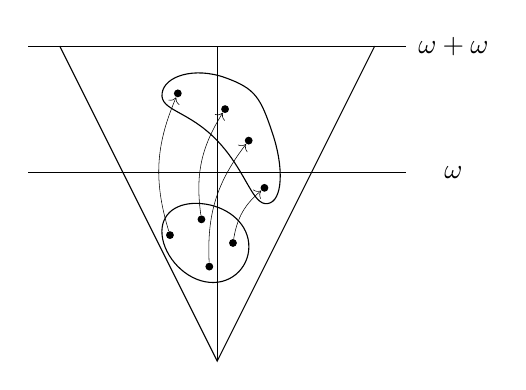
\begin{tikzpicture}[scale=2]
    \draw (1,2) -- (0,0) -- (-1,2);
    \draw (-1.2,2) -- (1.2,2);
    \draw [very thin] (-1.2,1.2) -- (1.2,1.2);
    \draw [very thin] (0,0) -- (0,2);
    \node at (1.5,2) {$\omega+\omega$};
    \node at (1.5,1.2) {$\omega$};
    \node [dot] (x1) at (-0.3,0.8) {};
    \node [dot] (x2) at (-0.05,0.6) {};
    \node [dot] (x3) at (0.1,0.75) {};
    \node [dot] (x4) at (-0.1,0.9) {};
    \draw plot [smooth cycle, tension=1] coordinates {(-0.35,0.8) (-0.05,0.5) (0.2,0.75) (-0.1,1)};
    \node [dot] (y1) at (-0.25,1.7) {};
    \node [dot] (y2) at (0.2,1.4) {};
    \node [dot] (y3) at (0.3,1.1) {};
    \node [dot] (y4) at (0.05,1.6) {};
    \draw [->, very thin] (x1) to[bend left=20] (y1);
    \draw [->, very thin] (x2) to[bend left=20] (y2);
    \draw [->, very thin] (x3) to[bend left=20] (y3);
    \draw [->, very thin] (x4) to[bend left=20] (y4);
    \draw plot [smooth cycle, tension=1] coordinates {(-0.35,1.7) (0.05,1.8) (0.35,1.45) (0.32,1.0) (0,1.4)};
  \end{tikzpicture}
\end{center}
\begin{idea}
  Take $x = \omega$, and
  \begin{equation*}
    F:
    \begin{cases}
      n \mapsto \omega + n \\
      y \mapsto 0 & \text{if } y \not\in \omega
    \end{cases}
  \end{equation*}
  Note $\omega+n$ is definable (in \hyperlink{def:axioms}{\textsf{Z}}): it is the unique \hyperlink{def:ordinal}{ordinal} which contains $\omega$ and $n-1$ elements above $\omega$.
\end{idea}
Let $Y \coloneqq \{F(n) \mid n \in \omega\}$. Then $\hyperlink{def:vk}{Y \subseteq V_{\omega+\omega}}$, but $Y \notin V_{\omega+\omega}$: it is not bounded in $V_{\omega+\omega}$.
\begin{center}
  \begin{tikzpicture}[scale=2]
    \draw (1,2) -- (0,0) -- (-1,2);
    \draw (-1.2,2) -- (1.2,2);
    \draw [very thin] (-1.2,1) -- (1.2,1);
    \draw [very thin] (0,0) -- (0,2);
    \node at (1.5,2) {$\omega+\omega$};
    \node at (1.5,1) {$\omega$};
    \draw [opacity=0.5, line width=3pt, line cap=round, bred] (0,0.75pt) -- (0, 1cm-0.75pt);
    \draw [opacity=0.5, line width=3pt, line cap=round, bblue] (0, 1cm+0.75pt) -- (0, 2cm-0.75pt);
    \foreach \x in {1,3,...,9}{
      \draw [->, bblue, thick] (0.5pt,\x*0.1) to[bend right=60] (0.5pt,1+\x*0.1);
    }
  \end{tikzpicture}
\end{center}
This example shows concretely that
\begin{equation*}
  V_{\omega + \omega} \models \neg \textsf{Repl.}
\end{equation*}

Similarly, if $\alpha$ is any \hyperlink{def:ordinal}{ordinal} such that there is a definable function $f: \omega \to \alpha$ such that the range of $f$ is unbounded in $\alpha$, then $V_\alpha \models \neg\textsf{Repl}$.
Even more generally, if $\beta < \alpha$ and a definable function $f: \beta \to \alpha$ with unbounded image, then $V_\alpha \models \neg\textsf{Repl}$.

\begin{defi}\hypertarget{def:reg}
  We call a cardinal $\kappa$ \named{regular} if there is no partition
  \begin{equation*}
    \kappa = \bigcup_{i \in I} A_i
  \end{equation*}
  such that $|I|, |A_i| < \kappa$ for all $i \in I$.
  Equivalently, for every $\alpha < \kappa$, there is no unbounded function $f: \alpha \to \kappa$.
\end{defi}

We know, e.g.\ that $\aleph_1$ is \hyperlink{def:reg}{regular}. Moreover, for any $\alpha$, $\aleph_{\alpha+1}$ is \hyperlink{def:reg}{regular}.
So our next candidate is $\alpha = \aleph_1$.

\begin{center}
  \begin{tikzpicture}[scale=2]
    \draw (1,2) -- (0,0) -- (-1,2);
    \draw (-1.2,2) -- (1.2,2);
    \draw [very thin] (-0.7,0.5) -- (0.7,0.5);
    \draw [very thin] (0,0) -- (0,2);
    \node at (1.5,2) {$\omega_1$};
    \node at (0.9,0.5) {$\omega$};
    \node [circle, fill=black, inner sep=1pt] at (-0.2, 0.6) {};
  \end{tikzpicture}
\end{center}
Note $\mathcal{P}(\omega) \in \hyperlink{def:vk}{V_{\omega+2}} \subseteq V_{\omega+1}$.
Clearly, there is a surjection
\begin{equation*}
  s: \mathcal{P}(\omega) \to \omega_1.
\end{equation*}
so the range of $s$ is unbounded in $\omega_1$.
Thus: $V_{\omega_1} \models \neg\textsf{Repl}$.

\begin{defi}\hypertarget{def:inacc}
  A cardinal $\alpha$ is called \named{inaccessible} if
  \begin{enumerate}[(a)]
    \item $\kappa$ is \hyperlink{def:reg}{regular}
    \item $\forall \lambda < \kappa$, $|\mathcal{P}(\lambda)| < \kappa$ \hypertarget{def:slim}(\named{strong limit}).
  \end{enumerate}
\end{defi}
That is, just take the two problems we had, negate them and make a definition.

\begin{remark}
  We know every successor cardinal is \hyperlink{def:reg}{regular}, and our simple examples of limit cardinals are all not regular: they were defined as unions.
  So, we can ask: `Are there regular limit cardinals?'
  (Such cardinals are sometimes called \named{weakly inaccessible}\index{inaccessible!weakly}).
  A partial answer: Under the Generalized Continuum Hypothesis ($\forall \kappa\ 2^\kappa = k^+$), we have:
  \begin{equation*}
    \kappa \text{ is \hyperlink{def:inacc}{inaccessible} } \iff \kappa \text{ is a regular limit cardinal}.
  \end{equation*}
\end{remark}

Now, let's assume that $\kappa > \aleph_0$ is \hyperlink{def:inacc}{inaccessible}.
\begin{lemma}
  \begin{equation*}
    \forall \lambda < \kappa \quad |\hyperlink{def:vk}{V_\lambda}| < \kappa.
  \end{equation*}
\end{lemma}
\begin{proof}
  Clearly $|\hyperlink{def:vk}{V_\omega}| = \aleph_0$, so $|V_\omega| < \kappa$.
  Proceed by induction. Suppose $|V_\lambda| < \kappa$. Then $V_{\lambda+1} = \mathcal{P}(V_\lambda)$.
  \begin{equation*}
  |V_{\lambda+1}| = |\mathcal{P}(V_\lambda)| < \kappa
  \end{equation*}
  by (b).
  Now let $\lambda < \kappa$ be a limit ordinal.
  Then
  \begin{equation*}
    V_\lambda = \bigcup_{\alpha < \lambda} V_\alpha.
  \end{equation*}
  Suppose for contradiction that $|V_\lambda| = \kappa$. But $|V_\alpha| < \kappa$ for all $\alpha < \kappa$, so you can write $\kappa$ as a union of $\lambda$ many things of smaller cardinality.
  This contradicts \hyperlink{def:reg}{regularity}.
\end{proof}

\begin{defi}[Mirimanoff rank]\hypertarget{def:rank}
  Define
  \begin{align*}
    \varrho(x) \coloneqq \text{least }\alpha\text{ such that }x \in V_{\alpha+1} \setminus V_\alpha.
  \end{align*}
\end{defi}
We prove useful properties about the \hyperlink{def:rank}{Mirimanoff rank} on question 4 on Example Sheet 1.

\begin{thm}
  If $\kappa$ is \hyperlink{def:inacc}{inaccessible}, then $\hyperlink{def:vk}{V_\kappa} \models \textsf{Repl}.$
\end{thm}
\begin{proof}
  Take any $F: \hyperlink{def:vk}{V_\kappa} \to V_\kappa$ and any $x \in V_\kappa = \bigcup_{\alpha < \kappa} V_\alpha$.
  Thus, find $\alpha < \kappa$ such that $x \in V_\alpha$.
  Since $V_\alpha$ is transitive, $x \subseteq V_\alpha$.
  So $|x| \leq |V_\alpha| < \kappa$ (by the lemma).

  Now consider $X \coloneqq \{F(y) \mid y \in x\}$.
  For each $y \in x$, we have $\hyperlink{def:rank}{\varrho(F(y))} < \kappa$ by assumption.
  Consider
  \begin{equation*}
  R \coloneqq \{\varrho(F(y)) \mid y \in x\},
  \end{equation*}
  then $|R| \leq |x| < \kappa$.
  By \hyperlink{def:reg}{regularity}, $\alpha \coloneqq \bigcup R < \kappa$.
  But then, $\forall y \in x \ F(y) \in V_{\alpha+1}$.
  So $X \subseteq V_{\alpha+1}$, $X \in V_{\alpha+2}$. This proves Replacement.
\end{proof}

Note we didn't even use that $F$ was definable: we showed a statement stronger than Replacement.
As a consequence, we get that the existence of \hyperlink{def:inacc}{inaccessible} cardinals cannot be proved in \hyperlink{def:axioms}{\textsf{ZFC}}:

\newlec \hypertarget{def:ic}Write \textsf{IC} for the axiom `there is an \hyperlink{def:inacc}{inaccessible} cardinal'.
If $\kappa$ is inaccessible, then $V_\kappa \models \textsf{ZFC}$.
$V_\kappa$ is a transitive model of \textsf{ZFC}, so,
\begin{equation*}
  \textsf{ZFC} + \textsf{IC} \vdash \underbrace{\text{`there is a transitive set that is a model of }\textsf{ZFC}\text{'}}_{\hyperlink{def:beta}{\beta}}
\end{equation*}
Recall that $\textsf{ZFC} + \cons{\textsf{ZFC}} \nvdash \beta$ from earlier, so $\textsf{ZFC} + \cons{\textsf{ZFC}} \nvdash \textsf{IC}$.

Now, recall from model theory:
\begin{enumerate}
  \item \named{L\"owenheim-Skolem Theorem}\hypertarget{thm:ls}:
    If $S$ is any structure in some countable first-order language $\mathcal{L}$ and $X \subseteq S$ is any subset, then there is a \named{Skolem hull} of $X$ in $S$,
    with $X \subseteq \mathcal{H}^S(X) \subseteq S$ such that
    \begin{enumerate}
      \item $\mathcal{H}^S(X) \preccurlyeq S$. \hypertarget{def:elsub}Recall $\preccurlyeq$ means \named{elementary substructure}, meaning that
        \begin{gather*}\forall \varphi \; \forall h_1, \dotsc, h_n \in \mathcal{H}^S(X), \\ \mathcal{H}^S(X) \models \varphi(h_1, \dotsc, h_n) \iff S \models \varphi(h_1, \dotsc, h_n)\end{gather*}
        \item
          $|\mathcal{H}^S(X)| \leq \max(\aleph_0, |X|)$
    \end{enumerate}
    \begin{proof}[Proof sketch]
      The key ingredient for this theorem is the \named{Tarski-Vaught criterion}, which says that for $Z \subseteq S$, we have $\hyperlink{def:elsub}{Z \preccurlyeq S}$ if and only if for every $\varphi$ and all $z_1, \dotsc, z_n$,
      \begin{equation*}
        S \models \exists x\; \varphi(x, z_1, \dotsc, z_n) \implies Z \models \exists x\; \varphi(x, z_1, \dotsc, z_n).
      \end{equation*}
      Observe there are $\max(\aleph_0, |X|)$ many possible $\varphi(x, z_1, \dotsc, z_n)$, so for each formula which we need to satisfy, take a witness in $S$ and add it into $X$.
      But this introduces new $z_i$, so we need to add more witnesses, so repeat this process and take a union. Specifically,
      \begin{align*}
        Z_0 &\coloneqq X \\
        Z_1 &\coloneqq Z_0 \cup \text{the witnesses for all tuples $\varphi, z_1, \dotsc, z_m$ where $z_1, \dotsc, z_m \in Z_0$} \\
        Z_{n+1} &\coloneqq Z_n \cup \text{the witnesses for all tuples $\varphi, z_1, \dotsc, z_m$ where $z_1, \dotsc, z_m \in Z_n$} \\
        Z &\coloneqq \bigcup_{n \in \mathbb{N}} Z_n.
      \end{align*}
      $Z$ is the required model. \qedhere
    \end{proof}

    Now, work in \hyperlink{def:axioms}{\textsf{ZFC}} + \hyperlink{def:ic}{\textsf{IC}}.
    Suppose $(M, \in) \models \textsf{ZFC} + \textsf{IC}$, which contains $\hyperlink{def:vk}{V_\kappa} \models \textsf{ZFC}$ ($V_\kappa \subseteq M$).
    Apply \hyperlink{thm:ls}{L\"owenheim-Skolem} to $V_\kappa$ with $X \coloneqq \emptyset$. Then
    \begin{equation*}
      H \coloneqq \mathcal{H}^{V_\kappa}(\emptyset) \preccurlyeq V_\kappa
    \end{equation*}
    and $\mathcal{H}^{V_\kappa}(\emptyset)$ has cardinality $\leq \aleph_0$, and $H \models \textsf{ZFC}$.

    There is a formula $\varphi$ such that $\varphi(x)$ iff $x$ is the least uncountable cardinal.
    We have $V_\kappa \models \exists x \ \varphi(x)$, since this is a theorem of \textsf{ZFC}, but the only element that satisfies $\varphi$ in $V_\kappa$ is $\aleph_1$.
    So in the notation of Skolem hull construction,
    \begin{equation*}
      \aleph_1 \in Z_1 \subseteq H
    \end{equation*}
    This implies $H$ can't be \hyperlink{def:transitive}{transitive}, since $\aleph_1$ has uncountably many elements, but $H$ has only countably many.
    So, try to collapse to a transitive model.
  \item \named{Mostowski Collapse Theorem}\hypertarget{thm:mct}:
    If $X$ is any set and $R \subseteq X \times X$ such that $R$ is well-founded and extensional, then there is a \hyperlink{def:transitive}{transitive} set $T$ such that $(T, \in) \cong (X,R)$.

    Consider $(H,\in) \models \hyperlink{def:axioms}{\textsf{ZFC}}$. Since $(H,\in) \models \textsf{ZFC}$, we must have that $\in$ is extensional on $H$.
    Since $\in$ (in $M$) is well-founded, $\in$ is well-founded on $H$.
    So, let $T$ be the \hyperlink{thm:mct}{Mostowski collapse} of $H$: $T$ is \hyperlink{def:transitive}{transitive} and
    \begin{equation*}
      (T,\in) \cong (H,\in).
    \end{equation*}
    But this is an isomorphism, so $(T,\in) \models \textsf{ZFC}$. It is a bijection also, so $|T| = |H| \leq \aleph_0$.

\end{enumerate}
Together: there is a countable \hyperlink{def:transitive}{transitive} model of \hyperlink{def:axioms}{\textsf{ZFC}}.

Notice that
\begin{align*}
  \varphi(x) &\coloneqq \text{`}x \text{ is countable'} \\
             &= \exists f \; (\underbrace{f: x \to \mathbb{N}}_{\hyperlink{def:delta0t}{\Delta_0^{\textsf{ZFC}}}}, \underbrace{f \text{ is injective}}_{\Delta_0^\textsf{ZFC}})
\end{align*}
is \hyperlink{def:sig1t}{$\Sigma_1^{\textsf{ZFC}}$}, so is \hyperlink{def:abso}{upwards absolute}.
But this formula is not \hyperlink{def:abso}{downwards absolute}: If $\alpha \in \textrm{Ord}$, $\alpha \in T$ then $\hyperlink{def:vk}{V_\kappa} \models \alpha$ is countable.
But since $(T,\in) \models \hyperlink{def:axioms}{\textsf{ZFC}}$, there is some $\alpha \in T$ such that $(T,\in) \models \alpha$ is uncountable, so $V_\kappa$ and $T$ disagree about the truth value of $\varphi(\alpha)$.

Consider now
\begin{align*}
  \psi(x) &\coloneqq  \text{`}x \text{ is a cardinal'} \\
  &= \forall \alpha \ (\alpha < x \rightarrow \text{there is no injection from $x$ to $\alpha$}).
\end{align*}
This is $\hyperlink{def:pi1t}{\Pi_1^{\textsf{ZFC}}}$.
In $(T,\in)$, take $\alpha$ least such that $(T,\in) \models \neg\varphi(\alpha)$.
Then $(T,\in) \models \text{`}\alpha$ is a cardinal'. Clearly, $\hyperlink{def:vk}{V_\kappa} \models \text{`}\alpha$ is not a cardinal'.

Note that if  $\lambda$ is an uncountable cardinal in $V_\kappa$, then $\lambda \notin T$, so the downwards absoluteness of $\psi$ is not very interesting.

So, try to ensure the cardinal is in $T$: Instead of building $\mathcal{H}^{V_\kappa}(\emptyset)$, build $H^* \coloneqq \mathcal{H}^{V_\kappa}(\omega_1 + 1)$.
Clearly $\omega_1 \in H^*$ and $\omega_1 \subseteq H^*$, so $\omega_1 \subseteq T^*$ and $\omega_1 \in T^*$. We have $|H^*| = \aleph_1$.

Now we have $V_\kappa \models \omega_1 \text{ is a cardinal}$, so by downwards absoluteness of $\psi$, so $T^* \models \omega_1$ is a cardinal.
But there may be other cardinals below $\omega_1$ in $T^*$, so it may not be the case that $T^* \models \omega_1 = \aleph_1$.

\newlec
In our goal to prove the \hyperlink{def:ch}{Continuum Hypothesis}, we have
\begin{enumerate}
  \item Decided to go for \hyperlink{def:transitive}{transitive models}
  \item Looked at `inner models'
  \item In particular, models of type \hyperlink{def:vk}{$V_\alpha$}
  \item Seen if $\alpha$ is \hyperlink{def:inacc}{inaccessible} then $V_\alpha \models \hyperlink{def:axioms}{\textsf{ZFC}}$
  \item Found countable transitive submodels $T \subseteq V$ such that $T \models \textsf{ZFC}$.
\end{enumerate}
But this isn't particularly helpful, since it is not going to change the truth value of CH.
If CH is true in our original model $(M,\in)$, then there is a bijection between $\mathbb{R}$ (or $\mathcal{P}(\mathbb{N})$) and $\omega_1$.
Certainly, $\mathbb{R} \in \hyperlink{def:vk}{V_{\omega+20}}$, and also $\omega_1 \in V_{\omega_1+1}$, and both of these are in $V_\kappa$.
So, the bijection is in $V_{\omega_1+20}$, certainly in $V_\kappa$.
This means
\begin{align*}
  (M,\in) \models \text{CH} \iff (V_\kappa, \in) \models \text{CH}
\end{align*}
By \hyperlink{thm:ls}{L\"owenheim-Skolem}, we found countable $H \preccurlyeq V_\kappa$, so
\begin{equation*}
  (H,\in) \models \text{CH} \iff (V_\kappa, \in) \models \text{CH}.
\end{equation*}
And \hyperlink{thm:mct}{Mostowski} had $(T,\in) \cong (H,\in)$ so
\begin{equation*}
  (T,\in) \models \text{CH} \iff (H, \in) \models \text{CH}.
\end{equation*}
In summary, the method of finding countable transitive elementary submodels of \hyperlink{def:vk}{$V_\kappa$} is not going to change the value of CH.

\subsubsection{Models of hereditarily small sets}
\begin{defi}\hypertarget{def:hered}
  Let $\kappa$ be a \hyperlink{def:reg}{regular} cardinal, e.g.\ $\kappa=\omega, \kappa=\omega_1$.
  Then $x$ is called \index{hereditary size}\textbf{hereditarily of size} $<\kappa$ if $|\tcl(x)| < \kappa$.
  Recall the \named{transitive closure}
  \begin{equation*}
    \hypertarget{def:tcl}\tcl(x) \coloneqq \bigcup_{m \in \mathbb{N}} t_n(x)
  \end{equation*}
  where
  \begin{align*}
    t_0(x) &\coloneqq x \\
    t_{n+1}(x) &\coloneqq \bigcup t_n(x).
  \end{align*}
\end{defi}
The definition of $|\hyperlink{def:tcl}{\tcl(x)}| < \kappa$ captures the intuition of
`$x$ has size $<\kappa$, all elements of $x$ have size $<\kappa$, all elements of elements of $x$ have size $<\kappa$, etc.'

Side remark: If $\kappa$ is not \hyperlink{def:reg}{regular}, this intuition might not work: Let $\kappa = \aleph_\omega$. Then define
\begin{align*}
  x_n^0 &\coloneqq \aleph_n \\
  x_n^{k+1} &\coloneqq \{x_n^k\} \\
  X &\coloneqq \{x_0^0, x_1^1, x_2^2, \dotsc\} \\
    &= \{\aleph_0, \{\aleph_1\}, \{\{\aleph_2\}\}, \{\{\{\aleph_3\}\}\},\dotsc\}
\end{align*}
$X$ is countable. In the notation from above,
\begin{equation*}
  |t_{n+1}(X)| = \aleph_n
\end{equation*}
But $|\tcl(X)| = \aleph_\omega$.

\begin{defi}
  \hypertarget{def:hk}Take $H_\kappa$ to be the sets which are \hyperlink{def:hered}{hereditarily of size $<\kappa$}.
\end{defi}

Observe
\begin{enumerate}
  \item \hyperlink{def:hk}{$H_\kappa$} is \hyperlink{def:transitive}{transitive}
  \item If $X \subseteq H_\kappa$ and $|X| < \kappa$, then $X \in H_\kappa$. (Follows directly from \hyperlink{def:reg}{regularity} of $\kappa$ and the definition).
\end{enumerate}

Take as our first example $\hyperlink{def:hk}{H_{\aleph_0}} \eqqcolon \hypertarget{def:hf}\hf$ (hereditarily finite)\index{hereditarily finite}.

\begin{prop}
$\hyperlink{def:hf}{\hf} = \hyperlink{def:vk}{V_\omega}$.
\end{prop}
\begin{proof}
  First show $\hyperlink{def:vk}{V_\omega} \subseteq \hyperlink{def:hf}{\hf}$.
  Need to show $V_n \subseteq \hf$ for all natural $n$.
  \begin{itemize}
    \item Clearly $V_0 = \emptyset \subseteq \hf$.
    \item If $V_n \subseteq \hf$ and $Z \subseteq V_n$, then by Observation 2, $Z \in \hf$ so $\mathcal{P}(V_n) = V_{n+1} \subseteq \hf$.
  \end{itemize}

  Next, we show $\hf \subseteq V_\omega$.
  Suppose not, then there are $x \in \hf \setminus V_\omega$.
  Take such an $x$ with minimal rank $\alpha$.
  Minimality says: If $y \in \hf$ with $\varrho(y) < \alpha$, then there is $k \in \mathbb{N}$ such that $\varrho(y) = k$.

  We have $x \in V_{\alpha+1} \setminus V_\alpha$, so $x \in \mathcal{P}(V_\alpha)$, $x \subseteq V_\alpha$.
  Also, $x \in \hf$, so $x$ is finite, say $x = \{x_1, \dotsc, x_n\}$.
  Using minimality, each $x_i$ is in $V_{k_i}$ for some natural $k_i$. So
  \begin{equation*}
    x \in V_{\max(k_1, \dotsc, k_n) + 1} \subseteq V_\omega
  \end{equation*}
  a contradiction.
\end{proof}
So we know $\hf \models \hyperlink{def:axioms}{\textsf{FST}}$.

Our next example of a regular cardinal was $\aleph_1$, so now try $H_{\aleph_1} \eqqcolon \hypertarget{def:hc}\hc$ (hereditarily countable\index{hereditarily countable}).
\begin{center}
  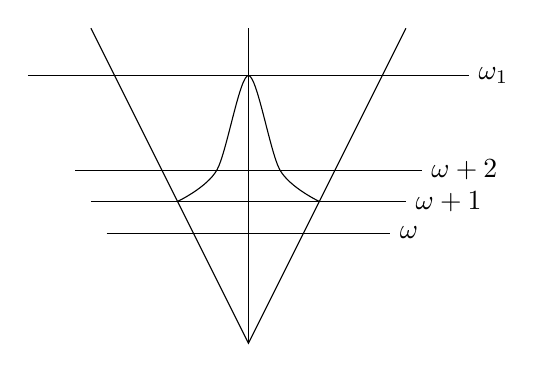
\begin{tikzpicture}[scale=2]
    \draw (1,2) -- (0,0) -- (-1,2);
    \draw [very thin] (-1.4,1.7) -- (1.4,1.7);
    \draw [very thin] (-1.1,1.1) -- (1.1,1.1);
    \draw [very thin] (-1.0,0.9) -- (1.0,0.9);
    \draw [very thin] (-0.9,0.7) -- (0.9,0.7);
    \draw [very thin] (0,0) -- (0,2);
    \node [right] at (1.4,1.7) {$\omega_1$};
    \node [right] at (1.1,1.1) {$\omega+2$};
    \node [right] at (1.0,0.9) {$\omega+1$};
    \node [right] at (0.9,0.7) {$\omega$};
    \draw plot [smooth] coordinates {(-0.45,0.9) (-0.2,1.1) (0,1.7) (0.2,1.1) (0.45,0.9)};
  \end{tikzpicture}
\end{center}
\begin{itemize}
  \item The ordinals in \hyperlink{def:hc}{\textit{HC}} are exactly $\omega_1$
  \item $\hyperlink{def:vk}{V_{\omega+2}} \setminus \hc \neq \emptyset$ (take, say, $\mathcal{P}(\mathbb{N})$)
  \item $V_{\omega+1} \subseteq \hc$
\end{itemize}
Which axioms are true in \hyperlink{def:hc}{\hc}?
\begin{description}
  \item[Pair] Take $x,y \in \hyperlink{def:hc}{\hc}$. $\{x,y\} \subseteq \hc$, $|\{x,y\}| < \aleph_1$, so $\{x,y\} \in \hc$.

    Separation and Union are similarly easy. Foundation follows trivially from foundation of the universe, and Extensionality follows by \hyperlink{def:transitive}{transitivity}.
    Replacement is harder:
  \item [Replacement] Let $F: \hyperlink{def:hc}{\hc} \to \hc$ and $x \in \hc$. Consider
    \begin{equation*}
      R \coloneqq \{F(y) \mid y \in x\} \subseteq \hc
    \end{equation*}
    then $|R| \leq |x| < \aleph_1$, and $R \subseteq \hc$ so by observation 2, $R \in \hc$.
  \item[Power Set] We know that $\mathbb{N} \in \hc$ and that $\mathcal{P}(\mathbb{N}) \notin \hc$. But this is not enough to show $\hc \models \neg \textsf{Pow}$.

    Instead, we need to show that for all $A \in \hc$,
    \begin{equation*}
      \hc \models `A \text{ is not the power set of } \mathbb{N}\text{'}
    \end{equation*}
    i.e.\
    \begin{equation*}
      \hc \models \exists X \ (X \subseteq \mathbb{N} \land X \notin A).
    \end{equation*}
    Fix $A \in \hc$ and presume that this might be the \hc-powerset of $\mathbb{N}$.
    Thus, if $X \subseteq \mathbb{N}$ and $X \in \hc$ then $X \in A$.

    But if $X \subseteq \mathbb{N}$, then $X \subseteq \hc$ and $|X| < \aleph_1$, so $X \in \hc$.
    So if $A$ is any set such that $\forall X\ (X \subseteq \mathbb{N} \text{ and } X \in \hc \rightarrow X \in A)$,
    then $A$ is uncountable, so $A \notin \hc$.
    Thus $\hc \models \neg \textsf{Pow}$.
\end{description}

\newlec
Using a similar result, we now have that \hyperlink{def:hk}{$H_\kappa$} is a model of all of \hyperlink{def:axioms}{\textsf{ZFC}} without Power Set if $\kappa$ is \hyperlink{def:reg}{regular}.
\begin{prop}
  If $\kappa$ is a \hyperlink{def:slim}{strong limit} cardinal, then $H_\kappa \models \textsf{Pow}$.
\end{prop}
\begin{proof}
  We'll show: if $x \in \hyperlink{def:vk}{H_\kappa}$, then $\mathcal{P}(x) \in H_\kappa$.
  This is much stronger than the Power Set axiom.
  \begin{equation*}
    \tcl(\mathcal{P}(x)) = \underbrace{\mathcal{P}(x)}_{\text{size } 2^{|x|} < \kappa} \cup \underbrace{\tcl(x)}_{\text{size} < \kappa}
  \end{equation*}
  Together, $|\tcl(\mathcal{P}(x))| < \kappa$, so $\mathcal{P}(x) \in H_\kappa$.
\end{proof}

\subsection{The Constructible Universe}
So far, all of our proofs were fairly crude: instead of forming the `internal' power set, we just used the external power set and showed it works.
Similarly for Replacement, we showed a much stronger statement.

So a more general idea would be to build inner models using `definability' properties, using the internal logic of a model.
The problem with this is that definability is not definable.
\begin{thm}[Tarski, Undefinability of truth]\hypertarget{thm:tarski}
  Let $(M,\in) \models \hyperlink{def:axioms}{\textsf{ZFC}}$. We assume that the language of set theory $\mathscr{L}_{\in} \subseteq M$.
  Consider the set $S$ of sentences in $\mathscr{L}_\in$ and the set $U$ of unary predicates ($\mathscr{L}_\in$-formulas in one free variable).
  \hypertarget{def:truthpred}A \named{truth predicate} would be a formula $T(x)$ in $\mathscr{L}_\in$ (i.e.\ $T \in U$) such that
  \begin{align*}
    (M,\in) \models \varphi \iff (M,\in) \models T(\varphi).
  \end{align*}
  There can be no such truth predicate.
\end{thm}
Contrast this with our previous result:
  If $M$ is a set, then `$(M,\in) \models \varphi$' is \hyperlink{def:delta0}{$\Delta_0$}.
\begin{proof}
  The key idea is diagonalisation.
  If $\varphi(x) \in U$, then we can ask whether
  \begin{equation*}
    \underbrace{\varphi(\varphi)}_{\in S}\text{ is true.}
  \end{equation*}
  Let's assume that $T$ is a \hyperlink{def:truthpred}{truth predicate}, and define
  \begin{equation*}\delta(x) \coloneqq \neg T(x(x))\end{equation*}
  where $x(x)$ is $x$ applied to $x$ if $x \in U$ and $\emptyset$ otherwise.
  Now apply $\delta$ to $\delta$, and note $ \delta(\delta) \in S $.
  \begin{equation*}
    M \models \delta(\delta) \iff M \models T(\delta(\delta))
  \end{equation*}
  since $T$ was a truth predicate, but also
  \begin{equation*}
    M \models \delta(\delta) \iff M \models \neg T(\delta(\delta)),
  \end{equation*}
  a contradiction.
\end{proof}

\begin{defi}
  \hypertarget{def:def}Again, let $M \models \textsf{ZFC}$. We say $x \in M$ is \named{definable} if there is a formula $\varphi$ such that
  \begin{equation*}
    \forall y \in M \quad x = y \iff M \models \varphi(y).
  \end{equation*}
  \hypertarget{def:dd}We say that a formula $D$ is called a \named{definition of definability} if
  \begin{equation*}
    \forall x \in M \quad x \text{ is definable} \iff M \models D(x).
  \end{equation*}
\end{defi}
\begin{thm}[Undefinability of definability]
  There is no formula $D$ that is a \hyperlink{def:dd}{definition of definability}.
\end{thm}
\begin{proof}
  Assume that $D$ is a \hyperlink{def:dd}{definition of definability}. Consider
  \begin{align*}
  \alpha \coloneqq \min\{\beta \mid \beta \text{ is not }\hyperlink{def:def}{\text{definable}}\text{ but } \forall \gamma < \beta \ \exists \gamma'\ \gamma < \gamma' < \beta \text{ and } \gamma' \text{ is definable} \},
  \end{align*}
  the supremum of the definable ordinals. This defined by the formula:
  \begin{equation*}
    y = \alpha \longleftrightarrow
    \begin{gathered}
    y \text{ is an ordinal and } \neg D(y) \text{ and }  \\
    \forall \gamma\ (\gamma < y \rightarrow \exists \gamma'\ (\gamma < \gamma' < y \land D(\gamma')))
    \end{gathered}
  \end{equation*}
  This proves that $\alpha$ is definable, so
  \begin{equation*}
    (M,\in) \models D(\alpha).
  \end{equation*}
  But one of the conjuncts in the definition implies $M \models \neg D(\alpha)$. Contradiction.
\end{proof}

We now learned that `definability' is not going to work without keeping track of parameters. So, we need to define `definability' with direct reference to what parameters are allowed.

\begin{defi}\hypertarget{def:defsubs}
  Fix $A$ and $m \in \mathbb{N}$. We're going to define by recursion what it means to be a \named{definable subset} of $A^n$:
  \begin{align*}
    \Diag_\in (A,n,i,j) &\coloneqq \{s \in A^n \mid s_i \in s_j\} \\
    \Diag_= (A,n,i,j) &\coloneqq \{s \in A^n \mid s_i = s_j\} \\
    \Proj(A,R,n) &\coloneqq \{s \in A^n \mid \exists t \in R\ (t \upharpoonright n = s)\} \\
    \Def(0,A,n) &\coloneqq \{\Diag_\in(A,n,i,j) \mid i,j < n\} \cup \{\Diag_=(A,n,i,j) \mid i,j < n\} \\
    \Def(k+1,A,n) &\coloneqq \Def(k,A,n)
    \begin{aligned}[t]
    &\cup \{R \cap S \mid R,S \in \Def(k,A,n)\} \\
    &\cup \{A^n \setminus S \mid S \in \Def(k,A,n)\} \\
    &\cup \{\Proj(A,R,n) \mid R \in \Def(k,A,n+1)\} \\
    \end{aligned} \\
    \Def(A,n) &\coloneqq \bigcup_{k \in \mathbb{N}} \Def(k,A,n).
  \end{align*}
\end{defi}

Observe the definitions of $\Def(k+1,A,n)$ and $\Def(0,A,n)$ are $\Delta_0$, so the definition of $\Def(A,n)$ is a recursive definition based on absolute notions and thus absolute for transitive models (containing $A$).

Next, use $\Def(A,n)$ to define the `definable power set'.
Note that $\Def(A,1)$ will be countable, so isn't a reasonable definition of the power set.
After that, define a `definable von Neumann hierarchy'.

\newlec
Our goal is to construct an inner model $L \subseteq M$ that is based on definability.
As we saw, this had problems, connected to \hyperlink{thm:tarski}{Tarski's Undefinability of Truth}.
The `definable' fragment of truth is that where we fix the scope of existential quantifiers in advance.

We recursively defined $\hyperlink{def:defsubs}{\Def(A,n)}$, the definable subsets of $A^n$ where definable is interpreted in $A$.

\begin{lemma}
  If $X \subseteq A^n$ such that there is a formula $\varphi$ such that
  \begin{align*}
    (x_1, \dotsc, x_n) \in X \iff (A,\in) \models \varphi(x_1, \dotsc, x_n)
  \end{align*}
  then $X \in \hyperlink{def:defsubs}{\Def(A,n)}$.
\end{lemma}
\begin{proof}
  Simple induction over complexity of $\varphi$.
\end{proof}
\begin{lemma}
  In $M$, we have that $\hyperlink{def:defsubs}{\Def(A,n)}$ is countable. (We even have a concrete surjection $\mathbb{N} \twoheadrightarrow \Def(A,n)$)
\end{lemma}
\begin{remark}
  In the definition of $\hyperlink{def:defsubs}{\Def(k,A,n)}$, we only used notions \hyperlink{def:abso}{absolute} for \hyperlink{def:transitive}{transitive} models of \hyperlink{def:axioms}{\textsf{ZF}}.
  So, since $\Def(A,n)$ was defined by recursion over $\Def(k,A,n)$, also $\Def(A,n)$ is absolute.
\end{remark}
\begin{aim}
  Our goal is to find a definable power set.
\end{aim}
\hyperlink{def:defsubs}{$\Def(A,1)$} is not a good candidate, since if $A$ is uncountable, then there is $a \in A$ such that $\{a\} \notin \Def(A,1)$ by the second lemma.
\begin{defi}\hypertarget{def:d}
  We define
  \begin{align*}
    \mathcal{D}(A) \coloneqq \left\{X \subseteq A\ \middle\vert\ \parbox{175pt}{\centering$\exists n\ \exists s \in A^n\ \exists R \in \hyperlink{def:defsubs}{\Def(A,n+1)}$ \\ s.t.\ $X = \{a \in A \mid (a,s_0, \dotsc, s_{n-1}) \in R\}$}\right\}
  \end{align*}
  We call this the \named{definable power set}.
\end{defi}
\begin{remark}\leavevmode
  \begin{enumerate}
    \item If $X$ is informally definable with parameters from $A$, i.e.\
      \begin{align*}
        X = \{a \in A \mid (A,\in) \models \varphi(a,\bar{p})\}
      \end{align*}
        with $\bar{p} \in A$, then $X \in \hyperlink{def:d}{\mathcal{D}(A)}$.
    \item As $\hyperlink{def:def}{\Def(A,n)}$ was \hyperlink{def:abso}{absolute} and the quantifiers in the definition of $\mathcal{D}(A)$ are all bounded, $\mathcal{D}(A)$ is absolute for \hyperlink{def:transitive}{transitive} models.
  \end{enumerate}
\end{remark}
\begin{prop}
  If $A$ is \hyperlink{def:transitive}{transitive}, then $\hyperlink{def:d}{\mathcal{D}(A)}$ is transitive.
\end{prop}
\begin{proof}
  Suppose $x \in X \in \hyperlink{def:d}{\mathcal{D}(A)}$. Then $x \in X \subseteq A$, so by \hyperlink{def:transitive}{transitivity} of $A$, $x \in A$.
  But since $x \in A$, we can define $x$ as a subset by the formula $v \in x = \varphi(v)$,
  \begin{equation*}
    x = \{z \in A \mid (A,\in) \models \varphi(z)\}. \qedhere
  \end{equation*}
\end{proof}
\begin{defi}
  \hypertarget{def:l}We can now define the \named{constructible hierarchy}.
  \begin{align*}
    L_0 &\coloneqq \emptyset \\
    L_{\alpha+1} &\coloneqq \mathcal{D}(L_\alpha) \\
    L_{\lambda} &\coloneqq \bigcup_{\alpha < \lambda} L_\alpha
  \end{align*}
  and we refer to the class $\bigcup_{\alpha \in \text{Ord}} L_\alpha$ as `$L$' or the `\named{constructible universe}'.
\end{defi}
\begin{enumerate}
  \item If $\alpha \leq \omega$, $\hyperlink{def:vk}{V_\alpha} = \hyperlink{def:l}{L_\alpha}$.
  \item For every $\alpha$, $L_\alpha$ is \hyperlink{def:transitive}{transitive} (follows from the proposition by induction).
  \item If $\alpha \leq \beta$ then $L_\alpha \subseteq L_\beta$.
  \item $\text{Ord} \cap L_\alpha = \alpha$.
  \item If $\alpha \geq \omega$ then $|L_\alpha| = |\alpha|$:
    \begin{proof}
      Induction. $\alpha=\omega$: $|L_\omega| = |V_\omega| = \aleph_0 = |\omega|$.
      Suppose for all $\beta < \alpha$ we have $|L_\beta| \leq |\beta|$.
      Show that $|L_\alpha| < |\alpha|^+$.
      \begin{itemize}
        \item If $\alpha=\beta+1$ is a successor, $L_\alpha = L_{\beta+1} = \mathcal{D}(L_\beta)$.
          Then there is a surjection from $\aleph_0 \times \bigcup_{n \in \mathbb{N}} L_\beta^n$ onto $\mathcal{D}(L_\beta)$, but $\aleph_0 \times \bigcup_{n \in \mathbb{N}} L_\beta^n$ has size $|L_\beta|$.
        \item If $\alpha$ is a limit, let $\pi_\beta: \alpha \to L_\beta$ be a surjection. Then we find surjection from $\alpha \times \alpha \twoheadrightarrow L_\alpha$, with $(\gamma,\gamma') \mapsto \pi_\gamma \gamma'$.
      \end{itemize}
      $|L_\alpha| \geq |\alpha|$ follows from 4.
    \end{proof}
  \item What about $V_{\omega+1}$ and $L_{\omega+1}$? $V_{\omega+1}$ is uncountable and $L_{\omega+1}$ is countable. $L_{\omega+1} \subseteq V_{\omega+1}$, and $V_{\omega+1} \setminus L_{\omega+1} \neq \emptyset$.
\end{enumerate}
\begin{defi}
  \hypertarget{def:lrank}If $x$ is constructible, $x \in L$, then
  \begin{equation*}
    \varrho_L(x) \coloneqq \min\{\alpha \mid x \in L_{\alpha+1}\}.
  \end{equation*}
\end{defi}
\begin{defi}
  \hypertarget{def:vl}$\textsf{V=L}$ is the \named{axiom of constructibility}, and refers to
  \begin{align*}
    \forall x\ \exists \alpha\ (x \in L_\alpha).
  \end{align*}
\end{defi}
This is a sentence in $\mathcal{L}_\in$.

Note that the formula describing `$x \in L_\alpha$' and `$x = L_\alpha$' are both \hyperlink{def:abso}{absolute} for \hyperlink{def:transitive}{transitive} models of set theory.

\begin{prop}
  If $A$ is a \hyperlink{def:transitive}{transitive} set model of \textsf{ZFC} + \hyperlink{def:vl}{\textsf{V=L}}, then there is a limit ordinal $\lambda$ such that $A = L_\lambda$.
\end{prop}
\begin{proof}
  \newlec
  Consider $\lambda \coloneqq \text{Ord} \cap A$. Clearly $\lambda$ is a limit ordinal (if not, $A$ thinks there is a largest ordinal, but $A \models \hyperlink{def:axioms}{\textsf{ZFC}}$).
  Claim that $A = \hyperlink{def:l}{L_\lambda}$.

  %Suppose that $x \in A$, by $V=L$ find $\alpha \in M$ such that $(M,\in) \models x \in L_\alpha$.
  %$L_\alpha$ was defined by recursion from absolute notions, so $x \in L_\alpha$ is absolute, so $x \in L_\alpha \subseteq L_\lambda$.
  %Suppose $x \in L_\lambda$, so there is $\alpha < \lambda$ such that $x \in L_\alpha$. By choice of $\lambda$, $\alpha \in M$, so by absoluteness, $(M,\in) \models x \in L_\alpha$.

  First show that $A \subseteq L_\lambda$. If $x \in A$, then by $(A,\in) \models \hyperlink{def:vl}{\textsf{V=L}}$, find $\beta$ such that $(A,\in) \models x \in L_\beta$. By \hyperlink{def:abso}{absoluteness}, $x \in L_\beta \subseteq L_\lambda$.

  Next show $L_\lambda \subseteq A$: If $x \in L_\lambda$, since $\lambda$ is a limit, $L_\lambda = \bigcup_{\beta < \lambda} L_\beta$ so find $\beta < \lambda$ and $x\in L_\beta$.
  Since $(A,\in) \models \textsf{ZFC}$, we know that there is $X$ such that $(A,\in) \models X = L_\beta$. By absoluteness, $X = L_\beta$.
  Therefore $L_\beta \in A$. $x \in L_\beta$, so by \hyperlink{def:transitive}{transitivity}, $x \in A$.
\end{proof}

Our next major goal is to show
\begin{thm}[G\"odel 1938]
If $\kappa$ is \hyperlink{def:inacc}{inaccessible}, then $\hyperlink{def:l}{L_\kappa} \models$ \hyperlink{def:axioms}{\textsf{ZFC}} + \hyperlink{def:vl}{\textsf{V=L}}.
\end{thm}
\begin{cor}
  If $\kappa$ is \hyperlink{def:inacc}{inaccessible}, then there is a countable $\alpha$ such that
  \begin{equation*}
    \hyperlink{def:l}{L_\alpha} \models \hyperlink{def:axioms}{\textsf{ZFC}} + \hyperlink{def:vl}{\textsf{V=L}}.
  \end{equation*}
\end{cor}
\begin{proof}
  Take $H \models \hyperlink{thm:ls}{\mathcal{H}}^{\hyperlink{def:l}{L_\kappa}}(\emptyset) \preccurlyeq \hyperlink{def:l}{L_\kappa}$. $H$ is countable.
  Take $T \cong H$ the \hyperlink{thm:mct}{Mostowski collapse}, $(T,\in) \equiv (L_\kappa, \in)$, so we have
  \begin{equation*}
    (T,\in) \models \hyperlink{def:axioms}{\textsf{ZFC}}+\hyperlink{def:vl}{\textsf{V=L}}
  \end{equation*}
  where $T$ is countable transitive.

  By the Proposition, $T=L_\alpha$ for some ordinal $\alpha$.
  By one of the earlier properties of $L$, we have $|L_\alpha| = |\alpha|$, so $\alpha$ is countable.
\end{proof}

Contrast this with: If $\hyperlink{def:vk}{V_\alpha} \models \hyperlink{def:axioms}{\textsf{ZFC}}$, then $\alpha$ cannot be countable:
If $\alpha$ is countable, there is a code for a surjection $f: \mathbb{N} \twoheadrightarrow \alpha$ in $V_{\omega+1} \subseteq V_\alpha$, so $V_\alpha \models $ `$\alpha$ is countable', contradicting $V_\alpha \models \textsf{ZFC}$.

\begin{proof}[Proof of G\"odel's Theorem]\leavevmode
  \begin{description}
    \item [Extensionality] Follows from \hyperlink{def:transitive}{transitivity}.
    \item[Pair] $x,y \in \hyperlink{def:l}{L_\kappa}$, find $\alpha$ such that $x,y \in L_\alpha$. $\{x,y\} \subseteq L_\alpha$.
      Clearly the formula $\varphi(z,x,y) \coloneqq z=x \land x=y$ defines the pair $\{x,y\}$, so by our Lemma earlier, the pair lies in $\hyperlink{def:d}{\mathcal{D}(L_\alpha)} = L_{\alpha+1} \subseteq L_\kappa$.

      The same proof takes care of, say, Union.
    \item [Power Set] Consider $x \in L_\kappa$.
      As before, $\alpha < \kappa$ with $x \in L_\alpha$.
      Since $L_\alpha$ is \hyperlink{def:transitive}{transitive}, $x \subseteq L_\alpha$. Then $|x| \leq |L_\alpha| < \kappa$, because $\kappa$ was \hyperlink{def:inacc}{inaccessible}.

      Consider $\mathcal{P}(x)$ in $M$,
      $|\mathcal{P}(x)| = 2^{|x|} < \kappa.$
      Now $|L_\kappa \cap \mathcal{P}(x)| \leq |\mathcal{P}(x)| < \kappa$.

        Since $L_\kappa$, $\mathcal{P}(x)$ are sets in $M$, $L_\kappa \cap \mathcal{P}(x)$ is a set in $V_\kappa$ and it is \hyperlink{def:defsubs}{definable} in $V_\kappa$ by the formula
        \begin{equation*}
          z \in L_\kappa \cap \mathcal{P}(x) \iff z \in L_\kappa \land z \subseteq x.
        \end{equation*}
        But that's not good enough to prove that $L_\kappa \cap \mathcal{P}(x) \in L_\kappa$.

      For each $z \in L_\kappa \cap \mathcal{P}(x)$ find $\alpha_z \coloneqq \hyperlink{def:lrank}{\varrho_L(z)} < \kappa$.
      Consider
      \begin{equation*}
      \{\alpha_z \mid z \in L_\kappa \cap \mathcal{P}(x)\} \subseteq \kappa,
      \end{equation*}
      of size $<\kappa$.
      By the regularity of $\kappa$, find a bound $\beta < \kappa$ such that
      \begin{equation*}
        \{\alpha_z \mid z \in L_\kappa \cap \mathcal{P}(x) \} \subseteq \beta
      \end{equation*}
      so $L_\kappa \cap \mathcal{P}(x) \subseteq L_\beta$.

      Define $\mathcal{P} \coloneqq \{z \mid (L_\beta, \in) \models z \subseteq x\}$. By our lemma, $\mathcal{P} \subseteq \mathcal{D}(L_\beta) = L_{\beta+1} \subseteq L_\kappa$.
      But $L_\kappa \models \forall z\ (z \in \mathcal{P} \iff z \subseteq x)$ so $L_\kappa \models \textsf{Pow}$.

    \item[Separation] \newlec Let $x \in \hyperlink{def:l}{L_\kappa}$, $\varphi$ a formula and take $a_1, \dotsc, a_n \in L_\kappa$.
      Separation says that (informally) $\{z \in x \mid \varphi(z,a_1, \dotsc, a_n)\}$ exists.
      More formally, we need to make the set
      \begin{equation*}
      \{z \in x \mid L_k \models \varphi(z, a_1, \dotsc, a_n)\}.
      \end{equation*}

      For each $1 \leq i \leq n$, find $\alpha_i < \kappa$ such that $a_i \in L_{\alpha_i}$ and find $\alpha < \kappa$ such that $x \in L_\alpha$.
      Define $\beta \coloneqq \max\{\alpha,\alpha_1, \dotsc, \alpha_n\}$.
      So for any $z \in x$, we have $z,a_1,\dotsc,a_n \in L_\beta$ by \hyperlink{def:transitive}{transitivity} of $L_\beta$.
      So
      \begin{align*}
        \{z \in x \mid L_\beta \models \varphi(z,a_1,\dotsc,a_n)\} \in \hyperlink{def:d}{\mathcal{D}(L_\beta)} = L_{\beta+1}.
      \end{align*}

      However, in general,
      \begin{align*}
        \{z \in x \mid L_\beta \models \varphi(z,a_1,\dotsc,a_n)\} \neq \{z \in x \mid L_\kappa \models \varphi(z,a_1,\dotsc,a_n)\}
      \end{align*}

    Consider $\hyperlink{thm:ls}{\mathcal{H}^{L_\kappa}(L_\beta)} \preccurlyeq L_\kappa$ with $|\mathcal{H}^{L_\kappa}(L_\beta)| = |L_\beta| = |\beta| < \kappa$.
    Now consider its \hyperlink{thm:mct}{Mostowski collapse}: $T \cong \mathcal{H}^{L_\kappa}(L_\beta)$ with Mostowski isomorphism $\pi: T \to \mathcal{H}^{L_\kappa}(L_\beta)$.
    $T$ is \hyperlink{def:transitive}{transitive}, $|T| = |\mathcal{H}^{L_\kappa}(L_\beta)| < \kappa$.

    \begin{equation*}
    \begin{tikzcd}
      T \rar{\pi}& \mathcal{H}^{L_\kappa}(L_\beta) \rar{\text{id}}& L_\kappa   \\
      \varphi(z,a_1, \dotsc, a_n) & \varphi(\pi(z),\pi(a_1),\dotsc,\pi(a_n)) & \varphi(\pi(z),\pi(a_1),\dotsc,\pi(a_n))
    \end{tikzcd}
    \end{equation*}

    We know that the Mostowski collapse is the identity on transitive sets. So if $X \subseteq L_\kappa$ is transitive, then $\pi \upharpoonright X = \text{id} \upharpoonright X$.

    Since $L_\beta$ is transitive and all $z, a_1, \dotsc, a_n$ are in $L_\beta$,
    \begin{align*}
      T \models \varphi(z,a_1, \dotsc, a_n) \iff L_\kappa \models \varphi(z,a_1, \dotsc, a_n).
    \end{align*}

    Run the `modified Skolem hull construction' from Example Sheet 1, Question 12.
    Set $\alpha_0 \coloneqq \text{Ord} \cap T$, and $\alpha_{n+1}$ as the least $\gamma$ such that $L_\gamma$ contains $L_{\alpha_n}$ and a witness for each existential statement true with parameters in $L_{\alpha_n}$.
    Then
    \begin{align*}
      \bar{\alpha} &\coloneqq \bigcup_{n \in \mathbb{N}} \alpha_{n} \\
      T &\preccurlyeq L_{\bar{\alpha}} \quad \text{with } \bar{\alpha} < \kappa.
    \end{align*}
    Define the set via $\varphi$ over $L_{\bar{\alpha}}$:
    \begin{align*}
      &\phantom{=}\,\ \ \!\!\{z \in x \mid L_{\bar{\alpha}} \models \varphi(z,a_1,\dotsc,a_n)\} \\
      &=\{z \in x \mid T \models \varphi(z,a_1,\dotsc,a_n)\} \\
      &=\{z \in x \mid \mathcal{H}^{L_\kappa}(L_\beta) \models \varphi(\pi(z),\pi(a_1),\dotsc,\pi(a_n))\} \\
      &=\{z \in x \mid \mathcal{H}^{L_\kappa}(L_\beta) \models \varphi(z,a_1,\dotsc,a_n)\} \\
      &=\{z \in x \mid L_\kappa \models \varphi(z,a_1,\dotsc,a_n)\}.
    \end{align*}
  \end{description}
  The rest of the axioms are similar.
\end{proof}
\begin{thm}[Condensation Lemma]\hypertarget{lem:con}
  If $\kappa$ is \hyperlink{def:inacc}{inaccessible} and $x,y \in \hyperlink{def:l}{L_\kappa}$, $y \subseteq x$ then there is an $\alpha< \kappa$ with
  \begin{align*}
    |\alpha| \leq |\hyperlink{def:tcl}{\tcl(x)}|
  \end{align*}
  such that $y \in L_\alpha$.
\end{thm}
\begin{proof}
  Let $t \coloneqq \hyperlink{def:tcl}{\tcl(x \cup \{y\})}$.
  Clearly $|t| = |\tcl(x)|$. Form $\hyperlink{thm:ls}{\mathcal{H}^{L_\kappa}(t)} \preccurlyeq \hyperlink{def:l}{L_\kappa}$.
  \hyperlink{thm:mct}{Mostowski collapse} the Skolem hull to
  \begin{equation*}
    T \xrightarrow{\pi} \mathcal{H}^{L_\kappa}(t) \preccurlyeq L_\kappa.
  \end{equation*}
  Now $|T| = |\mathcal{H}^{L_\kappa}(t)| = |t| = |\tcl(x)|$.
  $\pi$ is the identity on $t$, so $\pi(y) = y$ and $\forall z \in x$, $\pi(z) = z$ and $\pi(x) = x$.
  % The formula
  % \begin{align*}
  %   \forall z\ (z \in y \rightarrow z \in x).
  % \end{align*}

  By our lemma, find $\beta$ such that $T = L_\beta$, which we can do since $L_\kappa \models \textsf{ZFC}+\hyperlink{def:vl}{\textsf{V=L}}$, and $L_\beta \equiv L_\kappa$.
  Now $y$ can be defined over $L_\beta$ with parameters in $L_\beta$ (viz.\ $y$) and $|T| = |L_\beta| = |\beta|$.
\end{proof}

\begin{cor}
  \newlec
  If $x = \mathbb{N}$ and $y \subseteq \mathbb{N}$, then there is $\alpha < \omega_1$ such that $y \in \hyperlink{def:l}{L_\alpha}$.
\end{cor}
\begin{cor}\leavevmode
  \begin{enumerate}[(a)]
    \item $\mathcal{P}(\mathbb{N}) \cap \hyperlink{def:l}{L_\kappa} \subseteq L_{\omega_1}$.
      Observe that $\mathcal{P}(\mathbb{N}) \cap L_\kappa = \mathcal{P}^{L_\kappa}(\mathbb{N})$ where $\mathcal{P}^{L_\kappa}(\mathbb{N})$ refers to the unique $p \in L_\kappa$ such that $L_\kappa \models p = \mathcal{P}(\mathbb{N})$.
    \item $\mathcal{P}^{L_\kappa}(\mathbb{N}) \subseteq L_{\omega_1}$
    \item $|\mathcal{P}^{L_\kappa}(\mathbb{N})| \leq |L_{\omega_1}| = |\omega_1| = \aleph_1.$
  \end{enumerate}
\end{cor}
[A one-line proof of the \hyperlink{lem:con}{Condensation Lemma}:
\begin{align*}
  y \in \hyperlink{def:l}{L_\alpha} = \hyperlink{thm:mct}{T} \cong \hyperlink{thm:ls}{\mathcal{H}^{L_\kappa}}(\hyperlink{def:tcl}{\tcl(x)} \cup \{y\}) \preccurlyeq L_\kappa.
\end{align*}
]
Let's improve this to show $L_\kappa \models \hyperlink{def:ch}{\text{CH}}$.
The key idea is that $L_\kappa \models \hyperlink{def:axioms}{\textsf{ZFC}}$, then the \hyperlink{lem:con}{Condensation Lemma} is a theorem of \textsf{ZFC}, so apply Condensation Lemma inside $L_\kappa$.
But this is a lie! Our Condensation Lemma is a theorem of \textsf{ZFC}+\hyperlink{def:ic}{\textsf{IC}}.
\begin{remark}
  So if you assume \textsf{ZFC} + \textsf{2IC}, then this argument gets you that $L_\kappa \models \text{CH}$ for $\kappa$ the second inaccessible cardinal.
  This feels a bit odd. Let's try to do this without the second inaccessible.
\end{remark}
Work in $L_\kappa$. We know that $\mathcal{P}^{L_\kappa}(\mathbb{N}) \subseteq L_{\omega_1}$ where $\omega_1$ refers to the $\omega_1$ in $M$.
Note that $\omega_1 < \kappa$, $L_{\omega_1} \subseteq L_\kappa$.
\begin{align*}
  \mathcal{P}^{L_\kappa}(\mathbb{N}) \subseteq L_\beta = T \cong \mathcal{H}^{L_\kappa}(L_{\omega_1}) \preccurlyeq L_\kappa.
\end{align*}
By the standard argument, get
\begin{align*}
  \beta < \aleph_2 < \kappa.
\end{align*}
But now $L_\beta \models \textsf{ZFC}+\hyperlink{def:vl}{\textsf{V=L}}$.
Run the Condensation Lemma proof for $V_\kappa$ as $M$ and $L_\beta$ as $L_\kappa$:
\begin{equation*}
  y \in L_\alpha = T \cong \mathcal{H}^{L_\beta}(\mathbb{N} \cup \{y\}) \preccurlyeq L_\beta.
\end{equation*}
Now $L_\kappa \models$ `$a$ is countable'. So if $L_\kappa \models 2^{\aleph_0} \leq \aleph_1$ then $L_\kappa \models \hyperlink{def:ch}{\text{CH}}$.
\begin{thm}
  $\cons(\hyperlink{def:axioms}{\textsf{ZFC}}+\hyperlink{def:ic}{\textsf{IC}}) \implies \cons(\textsf{ZFC}+\hyperlink{def:ch}{\text{CH}})$.
\end{thm}
\begin{remark}\leavevmode
  \begin{enumerate}[(1)]
    \item The same argument with $x=\lambda$ for some $L_\kappa$-cardinal $\lambda$ gives us $L_\kappa \models 2^\lambda \leq \lambda^+$. So GCH holds: $\forall \lambda, 2^\lambda = \lambda^+$.
    \item What about the inaccessible?
      \begin{enumerate}[(a)]
        \item If we have a \hyperlink{def:transitive}{transitive} set model of \hyperlink{def:axioms}{\textsf{ZFC}} then we can mimic this proof.
        \item There is a way of getting around that assumption as well:
          Use the L\'evy Reflection Theorem (Example sheet 2):
          Fix in advance some finite list $\Phi$ of sentenes you wish to preserve and find sufficiently large $\alpha$ such that $\Phi$ is absolute for $V_\alpha$.

          Go through all needed absoluteness results and lemmas and collect for each of them $\varphi$ the finite set $\Phi_\phi$ of axioms of \textsf{ZFC} needed to prove them. Form $\Phi = \bigcup_{\phi} \Phi_\phi$, a finite union over all the relevant $\phi$.
          Apply L\'evy to $\Phi$ and run the previous proof to get a model of $\Phi + \text{CH}$.
          Now consider all finite subsets $\Psi$ such that $\Phi \subseteq \Psi \subseteq \textsf{ZFC}$ and get models of $\psi$+CH.
          Compactness gives a model of \textsf{ZFC}+\text{CH}.
      \end{enumerate}
    \item Consider
      \begin{equation*}
        L = \bigcup_{\alpha \in \text{Ord}} L_\alpha \subseteq M.
      \end{equation*}
      Our proof does not say what axioms hold in $L$, but using the L\'evy Reflection Theorem, you can prove that $V \models \textsf{ZFC}$, then $L \models \textsf{ZFC}+\hyperlink{def:vl}{\textsf{V=L}}$.
  \end{enumerate}
\end{remark}
Recall our question about regular limit cardinals:
We have two notions: regular/singular and successor/limit.

\begin{center}
\begin{tabular}{c|cc}
  & Reg & Sing \\ \hline
  succ & \cmark & \xmark \\
  limit & ? & \cmark
\end{tabular}
\end{center}
If we strengthen `limit' ($\forall \lambda < \kappa\  (\lambda^+ < \kappa)$) to `\hyperlink{def:slim}{strong limit}' ($\forall \lambda < \kappa\ (2^\lambda < \kappa)$), then we showed that \hyperlink{def:axioms}{\textsf{ZFC}} cannot prove the existence of \hyperlink{def:reg}{regular} strong limits = \hyperlink{def:inacc}{inaccessible} cardinals.
Clearly \textsf{ZFC}+GCH gives that every limit is a strong limit. So, \textsf{ZFC}+GCH gives that every regular limit is an inaccessible cardinal.
\begin{proof}
  Assume that $M \models \hyperlink{def:axioms}{\textsf{ZFC}}$ and that $\textsf{ZFC} \vdash$ there are \hyperlink{def:reg}{regular} limits.
  Towards a contradiction with G\"odel's Incompleteness Theorem, prove $M \models \cons(\textsf{ZFC})$.
  Consider $L \subseteq M$. Then by remark (3), $L \models \textsf{ZFC}$+GCH.
  By $\textsf{ZFC}\vdash \exists$ regular limit, we get $L \models \textsf{ZFC}+\text{GCH}+\exists \kappa$ regular limit. Thus, $L \models \textsf{ZFC}+\hyperlink{def:ic}{\textsf{IC}}$.
  Then $L \models \exists \kappa (L_\kappa \models \textsf{ZFC})$, so $L \models \cons(\textsf{ZFC)})$ thus $M \models \cons(\textsf{ZFC})$ by absoluteness, a contradiction.
\end{proof}

\subsection{The limitations of the method of inner models}
\begin{defi}\hypertarget{def:innerModel}
  \newlec
  If $(M,\in) \models \hyperlink{def:axioms}{\textsf{ZFC}}$ and $N \subseteq M$, we say that $N$ is an \named{inner model} of $M$ if
  \begin{enumerate}[(a)]
    \item $(N,\in) \models \textsf{ZFC}$
    \item $\text{Ord} \cap N = \text{Ord} \cap M$
    \item $N$ is \hyperlink{def:transitive}{transitive} in $M$.
  \end{enumerate}
\end{defi}
\begin{thm}[Minimality Theorem]\hypertarget{thm:min}
  If $M \models \textsf{ZFC} + \hyperlink{def:vl}{\textsf{V=L}}$ and $N$ is an \hyperlink{def:innerModel}{inner model} then $N = M$.
\end{thm}
\begin{proof}
  We know that $M = \bigcup_{\alpha \in \text{Ord} \cap M} L_\alpha^{M}$ where $L_\alpha^M$ is the set $L_\alpha$ (interpreted in $M$).
  This follows directly from $\hyperlink{def:vl}{\textsf{V=L}}$ in $M$.
  So in order to show $N=M$, it's enough to show $L_\alpha^M \subseteq N$ for all $\alpha \in \text{Ord} \cap M$.
  An easy induction shows $L_\alpha^N \subseteq N$ for $\alpha \in \text{Ord} \cap N$. By absoluteness $L_\alpha^N = L_\alpha^M$
\end{proof}
\begin{remark}\leavevmode
  \begin{enumerate}
    \item If you drop (b), you still get $N = L_\Omega^M$ where $\Omega = \text{Ord} \cap N$.
    \item Of course, we don't even need full \hyperlink{def:axioms}{\textsf{ZFC}} for this.
  \end{enumerate}
\end{remark}
The `technique of inner models' is then:
\begin{itemize}
  \item Want to show $\cons(\hyperlink{def:axioms}{\textsf{ZFC}}+\varphi)$
  \item Start with $M \models \textsf{ZFC} + \neg \varphi$
  \item Go to an inner model $N \subseteq M$, where $N \models \textsf{ZFC} +\varphi$.
\end{itemize}
\begin{defi}
  A \named{definable inner model}\index{inner model!definable} is an $L_\in$-formula $\Phi$ with one free variable with the property: if $(M,\in) \models \hyperlink{def:axioms}{\textsf{ZFC}}$, then define
  \begin{align*}
    N \coloneqq \{x \in M \mid M \models \Phi(x)\}.
  \end{align*}
  Then $N$ is an \hyperlink{def:innerModel}{inner model} of $M$.
\end{defi}
\begin{eg}
  $L$ `is' such an inner model. We mean $\Phi(x) \vcentcolon\leftrightarrow \exists \alpha\ (x \in L_\alpha)$.
\end{eg}
Now we can define what we mean by
`the consistency of $\varphi$ can be shown by inner models'
This means: We find an inner model $\Phi$ such that for all $M \models \hyperlink{def:axioms}{\textsf{ZFC}}$ and
\begin{align*}
N \coloneqq \{x \in M \mid M \models \Phi(x)\},
\end{align*}
$N \models \textsf{ZFC}+\varphi$.
\begin{cor}
  There is no \hyperlink{def:innerModel}{inner models} proof of the consistency of $\neg$\hyperlink{def:ch}{CH}.
\end{cor}
\begin{proof}
  Suppose otherwise, so let $\Phi$ be an inner model that proves consistency of $\neg$\hyperlink{def:ch}{CH}.
  Take an arbitrary $M \models \hyperlink{def:axioms}{\textsf{ZFC}}$. Build $L^M$ and form
  \begin{align*}
  N^* \coloneqq \{x \in L^M \mid L^M \models \varphi(x)\}.
  \end{align*}
  This is an inner model of $L^M$, thus by minimality $N^* = L^M$. So, $N^* \models \neg\text{CH} \land \text{CH}$.
  Contradiction.
\end{proof}

\clearpage
\section{Outer models}
So, try outer models.
As an illustration, take $\mathcal{L}$ the language of arithmetic $+,\cdot,0,1$.
Take $\text{FLD}$, the axioms of fields, and $\Phi_0$ the axiom (schema) for characteristic zero, and $\text{FLD}_0 \coloneqq \text{FLD}+\Phi_0$, fields of characteristic $0$.

Each characteristic has a prime field $\mathbb{Q}$. $\mathbb{Q}$ is minimal in the sense that it has no proper subfields.

\begin{equation*}
  \text{NSRT} \coloneqq \forall x\ (x \cdot x \neq 1 + 1)
\end{equation*}
We know $Q \models \text{NSRT}$ (there is No Square Root of Two).
In analogy to the discussion of \hyperlink{def:innerModel}{inner models}, the technique of submodels cannot show $\cons(\text{FLD}_0 + \neg\text{NSRT})$
So, we use outer models. Find $X \notin \mathbb{Q}$ (from the surrounding meta-universe), with $X^2 = 2$.
We can't just take $\mathbb{Q} \cup \{X\}$, since it may not be a model of $\text{FLD}_0$, so we close under the field axioms: we need $X+X$, $X+X+X$, $q \cdot X$, $X^3$ and so on.
Algebra has various techniques that allow us to do constructions and obtain $\mathbb{Q}(X) \models \text{FLD}_0+\neg\text{NSRT}$.
\medskip

Back to set theory: Suppose we have a countable \hyperlink{def:transitive}{transitive} $M \models \hyperlink{def:axioms}{\textsf{ZFC}}+\hyperlink{def:ch}{\textsf{CH}}$.
Then all of its elements are countable: $\mathbb{R}^M, \aleph_1^M, \aleph_2^M, \aleph_3^M$ and so on.
Since $\mathbb{R}^M$ is countable, there are lots of reals not in $M$.

In particular, there is an injection $i: \aleph_2^M \to \mathbb{R}$ such that the range of $i$ is disjoint from $M$.
Now form $M(i)$, the smallest $\textsf{ZFC}$-model containing $M$ as a subset and $i$ as an element (we have not yet formally defined this, but pretend for now that we have a technique to do so).
Now $M(i) \models \textsf{ZFC} + (|\mathbb{R}| \geq |\aleph_2^M|)$.

Unfortunately, $\neg$\textsf{CH} would need $|\mathbb{R}| \geq |\aleph_2^{M(i)}|$.
So, we additionally need $\aleph_1^M = \aleph_1^{M(i)}$ and $\aleph_2^M = \aleph_2^{M(i)}$ in order to get this.

Thus our proof components are:
\begin{enumerate}
  \item Find a construction of $M(i) \models \textsf{ZFC}$
  \item Preservation theorems for cardinals
\end{enumerate}
Our only preservation theorem so far: $\mathbb{R}^M = \mathbb{R}^N \Rightarrow \aleph_1^M = \aleph_1^N$ (Example Sheet question 10).

General problem: If $x$ codes a well order on $\mathbb{N}$ of order type $\aleph_1^M$ and $i(\gamma) = x$ then $M(i) \models \aleph_1$ is countable.

\newlec
So, in the meta-universe, we have $i : \aleph_2^M \to \mathbb{R}$, and we would like
\begin{enumerate}
  \item $M[i] \models \hyperlink{def:axioms}{\textsf{ZFC}}$ \hyperlink{def:transitive}{transitive}, with $M \subseteq M[i]$ and $i \in M[i]$.
  \item $\aleph_2^{M[i]} = \aleph_2^M$. This is stronger than $\aleph_1^{M[i]} = \aleph_1^M$.
\end{enumerate}
We had the issue that if $x$ is in the range of $i$, then $x \in M[i]$.
If $x$ is a code for the countability of $\aleph_1^M$, then $M[i] \nModels \aleph_2^{M[i]} = \aleph_2^M$.

Even worse: if such an $x$ can be constructed in \textsf{ZFC} from $i$, then it will be in $M[i]$.
So, we need to guarantee that no such objects can be constructed.

With this goal, Paul Cohen described \named{Forcing} in 1963.

\begin{defi}\leavevmode
  \begin{itemize}
    \item \hypertarget{def:poset}As usual, we call $(\mathbb{P}, \leq, \mathbbm{1})$ a \named{partial order}/forcing/forcing partial order if $\mathbb{P}$ is a set, $\leq$ is a reflexive, transitive, antisymmetric relation, and $\mathbbm{1}$ is the largest element.
    \item Elements of $\mathbb{P}$ are called \named{conditions}
      \begin{center}
        $p \leq q$ is read as `$p$ is stronger than $q$'
      \end{center}
    \item \hypertarget{def:chain}As usual, $C \subseteq \mathbb{P}$ is called a \named{chain} if $(C, \leq)$ is a total order.
    \item \hypertarget{def:incompat}If $p,q \in \mathbb{P}$, say that $p$ and $q$ are \named{incompatible}, written $p \perp q$ if there is no $r \leq p,\ r \leq q$.
    \item \hypertarget{def:antichain}$A \subseteq \mathbb{P}$ is called an \named{antichain} if
      \begin{align*}
        \forall p,q \in A \text{ if } p \neq q \rightarrow p \perp q.
      \end{align*}
    \item \hypertarget{def:ccc} We say that $\mathbb{P}$ has the \named{countable chain condition} (ccc) if every antichain $\mathbb{P}$ is countable.
    \item \hypertarget{def:dense}If $D \subseteq \mathbb{P}$, we say $D$ is \named{dense} if
      \begin{align*}
        \forall p \in \mathbb{P}\ \exists q \in D\ q \leq p
      \end{align*}
    \item \hypertarget{def:filter}If $F \subseteq \mathbb{P}$, we say $F$ is a \named{filter} if
      \begin{enumerate}[(a)]
        \item $\forall p \in F \ \forall q\ (q \geq p \rightarrow q \in F)$
        \item $\forall p,q \in F \ \exists r \in F \ r \leq p,q$.
      \end{enumerate}
    \item \hypertarget{def:splitting}We say that $\mathbb{P}$ is \named{splitting} if for all $p \in \mathbb{P}$
      \begin{align*}
        \exists q_1,q_2 \in \mathbb{P} \ q_1,q_2 \leq p \text{ and } q_1 \perp q_2.
      \end{align*}
    \item \hypertarget{def:dgeneric}If $\mathcal{D}$ is a set of dense sets and $G \subseteq \mathbb{P}$, we say that $G$ is $\mathcal{D}$-\named{generic} if $\forall D \in \mathcal{D}$, $D \cap G \neq \emptyset$.
  \end{itemize}
\end{defi}

\begin{eg}[Cohen forcing]
  \begin{align*}
    \mathbb{P} &\coloneqq \{p \mid p\text{ is a partial function from }\mathbb{N}\text{ to }2\text{ with finite domain}\} \\
    p \leq q &:\Leftrightarrow p \supseteq q \\
    \mathbbm{1} &\coloneqq \emptyset
  \end{align*}
  Note that if $p \hyperlink{def:incompat}{\perp} q$, then there is $n \in \dom(p) \cap \dom(q)$ such that $p(n) \neq q(n)$.
  If $F$ is a \hyperlink{def:filter}{filter} in $\mathbb{P}$, then $\bigcup F$ is a partial function from $\mathbb{N}$ into $2$.
  Consider $D_n \coloneqq \{p : n \in \dom(p)\}$.
  This is \hyperlink{def:dense}{dense} in $\mathbb{P}$.
  Set $\mathcal{D} \coloneqq \{D_n : n \in \mathbb{N}\}$.
  If $F$ is \hyperlink{def:dgeneric}{$\mathcal{D}$-generic}, then $\bigcup F: \mathbb{N} \to 2$.
\end{eg}
\begin{eg}
  Take now
  \begin{align*}
    \mathbb{P}_X &\coloneqq \{p \mid p\text{ is a partial function from }\mathbb{N}\text{ to }X\text{ with finite domain}\}
  \end{align*}
  for $X$ any set.
  As before, if $F$ is a \hyperlink{def:filter}{filter}, $\bigcup F$ is a partial function.
  If $F$ is \hyperlink{def:dgeneric}{$\mathcal{D}$-generic}, $\bigcup F: \mathbb{N} \to X$.

  Consider $E_x \coloneqq \{p \mid x \in \ran(p)\}$ for every $x \in X$.
  \begin{align*}
    \mathcal{D}^* \coloneqq \mathcal{D} \cup \{E_x \mid x \in X\}.
  \end{align*}
  Suppose $G$ is a $\mathcal{D}^*$-generic filter. By the above, $\bigcup G: \mathbb{N} \to X$.
  For every $x \in X$, $E_x \cap G \neq \emptyset$, so there is $p \in G$ with $x \in \ran(p)$.
  So $X = \ran(\bigcup G)$.
  Thus $\bigcup G$ is a surjection from $\mathbb{N}$ to $X$. % (In particular, if $X$ is uncountable in $M$, there is no such generic filter).
\end{eg}
\begin{defi}\hypertarget{def:genericO}
  If $M$ is a \hyperlink{def:transitive}{transitive} model of \hyperlink{def:axioms}{\textsf{ZFC}} and $\mathbb{P} \in M$ a \hyperlink{def:poset}{partial order}.
  We say that a \hyperlink{def:filter}{filter} $G$ (not necessarily an element of $M$) is \named{generic over $M$} if it is \hyperlink{def:dgeneric}{$\mathcal{D}$-generic} for $\mathcal{D} \coloneqq \{D \in M \mid D \text{ is dense in } \mathbb{P}\}$.
\end{defi}
\begin{lemma}
  Suppose $\mathbb{P}$ is \hyperlink{def:splitting}{splitting}, $\mathbb{P} \in M$ and $M$ is a \hyperlink{def:transitive}{transitive} model of \hyperlink{def:axioms}{\textsf{ZFC}}.
  Suppose $G$ is a $\mathbb{P}$-\hyperlink{def:genericO}{generic filter over $M$}. Then $G \notin M$.
\end{lemma}
\begin{proof}
  Suppose $G \in M$. Then $D \coloneqq \mathbb{P} \setminus G \in M$. We claim that $D$ is \hyperlink{def:dense}{dense}.
  Take $p \in \mathbb{P}$ arbitrary. $\mathbb{P}$ is \hyperlink{def:splitting}{splitting}, so we find $q_1,q_2 \leq p$ with $q_1 \perp q_2$.
  Since $G$ is a \hyperlink{def:filter}{filter}, not both $q_1, q_2 \in G$, so at least one is in $D$.
  So by definition $G \cap D = G \cap \mathbb{P} \setminus G \neq \emptyset$, a contradiction.
\end{proof}
\begin{lemma}
  \newlec
  If $\mathcal{D}$ is a countable set of \hyperlink{def:dense}{dense} sets and $p \in \mathbb{P}$, then there is a \hyperlink{def:dgeneric}{$\mathcal{D}$-generic} \hyperlink{def:filter}{filter} $G$ in $\mathbb{P}$ such that $p \in G$.
\end{lemma}
\begin{proof}
  Let $\mathcal{D} = \{D_n \mid n \in \mathbb{N}\}$.
  Define $p_0 \coloneqq p$. Suppose $p_0 \geq \dotsb \geq p_n$ are already defined.
  By definition, $D_n$ has an element $q$ such that $q \in D_n$, $q \leq p_n$. Then $p_{n+1} \coloneqq q$.

  Consider $X \coloneqq \{p_n \mid n \in \mathbb{N}\} \subseteq \mathbb{P}$.
  Note that if $p_n, p_k \in X$ then $p_{\max(n,k)} \leq p_n,p_k$.
  So $G \coloneqq \{p \mid \exists n \ p_n \leq p\}$ is a \hyperlink{def:filter}{filter} on $\mathbb{P}$.
  Clearly, for every $n$, $G \cap D_n \neq \emptyset$, as required.
\end{proof}
\begin{cor}
  If $M$ is a countable \hyperlink{def:transitive}{transitive} model of set theory, $p \in \mathbb{P} \in M$.
  Then there is a \hyperlink{def:dgeneric}{$\mathbb{P}$-generic} \hyperlink{def:filter}{filter} $G$ \hyperlink{def:genericO}{over $M$} with $p \in G$.
\end{cor}
\begin{proof}
  $\mathbb{P} \in M$, then $\mathbb{P}$ is countable.
  \begin{align*}
    \{D \subseteq \mathbb{P} \mid D \text{ is dense, } D \in M\} \subseteq \mathcal{P}^M(\mathbb{P})
  \end{align*}
  so this is countable as well.
\end{proof}

\subsection{Forcing language}
\begin{defi}
Fix $M$ a \hyperlink{def:transitive}{transitive} model of set theory, $\mathbb{P} \in M$.
\begin{align*}
  \hypertarget{def:name}\name_0(M, \mathbb{P}) &\coloneqq \emptyset \\
  \lambda> 0 \quad \name_\lambda(M, \mathbb{P}) &\coloneqq \left\{\tau\ \middle\vert \parbox{23em}{\centering each element of $\tau$ is an ordered pair $(\sigma,p)$ \\ where $\sigma \in \name_\alpha(M,\mathbb{P})$ for some $\alpha < \lambda$ and $p \in \mathbb{P}$}\right\}
\end{align*}
The elements of
\begin{align*}
  M^{\mathbb{P}} \coloneqq\ \bigcup_{\mathclap{\lambda \in \text{Ord} \cap M}}\ \name_\lambda(M,\mathbb{P})
\end{align*}
are called $\mathbb{P}$-\named{names}.
\end{defi}

\begin{eg}[Silliest example]
  Take $\mathbb{P} = \{1\}$.
  Then $\emptyset$ is a \hyperlink{def:name}{name}, so $\{(\emptyset,\mathbbm{1})\}$ is a name.
  This results in (an isomorphic copy) of the \hyperlink{def:vk}{von Neumann hierarchy} inside $M$.
\end{eg}
\begin{eg}[Silly example]
  Take the following \hyperlink{def:poset}{partial order}:
  \begin{center}
    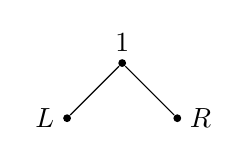
\begin{tikzpicture}[every node/.style={inner sep=1pt, fill=black, circle}, scale=0.7]
      \node [label=left:$L$] (L) at (-1,0) {};
      \node [label=right:$R$] (R) at (1,0) {};
      \node [label=above:$\mathbbm{1}$] (1) at (0,1) {};
      \draw (L) -- (1) -- (R);
    \end{tikzpicture}
  \end{center}
  \begin{itemize}
    \item What are the \hyperlink{def:dense}{dense sets}? $\{\mathbbm{1},L,R\}, \{L,R\}$.
    \item What is a \hyperlink{def:filter}{filter}? $\{\mathbbm{1}\}, \{\mathbbm{1},L\}$ and $\{\mathbbm{1},R\}$.
    \item What does \hyperlink{def:genericO}{generic} mean? Meets every dense set, so contains $L$ or $R$. Hence $\{\mathbbm{1},L\}$, $\{\mathbbm{1},R\}$ are the generic filters.
  \end{itemize}
  Now, $\emptyset$ is a \hyperlink{def:name}{name}.
  On the next level, the relevant ordered pairs are $(\emptyset, \mathbbm{1})$, $(\emptyset, L)$, $(\emptyset,R)$.
  So, the new names at level 1 are
  \begin{gather*}
    \{(\emptyset,\1)\}, \{(\emptyset,L)\}, \{(\emptyset,R)\} \\
    \{(\emptyset,\1), (\emptyset,L)\}, \{(\emptyset,\1), (\emptyset,R)\}, \{(\emptyset,L), (\emptyset,R)\} \\
    \{(\emptyset,\1), (\emptyset,L), (\emptyset,R)\}
  \end{gather*}
\end{eg}

Now that we have these names, we would like to interpret them.
\begin{defi}
  Let $\mathbb{P}, M$ be as before and let $G$ be \hyperlink{def:genericO}{$\mathbb{P}$-generic over $M$}, $G \subseteq \mathbb{P}$.
  If $\tau \in \name(M,\mathbb{P})$, I define the $G$-\named{value} of $\tau$:
  \begin{align*}
    \hypertarget{def:val}\val(\tau,G) \coloneqq \{\val(\sigma,G) \mid \exists p \in G, (\sigma,p) \in \tau\}.
  \end{align*}
  Define also
  \begin{align*}
    \hypertarget{def:mg}M[G] \coloneqq \{\val(\tau,G) \mid \tau \in \name(M,\mathbb{P})\}.
  \end{align*}
\end{defi}

\begin{observation}
  If $N$ is a \hyperlink{def:transitive}{transitive} model of \hyperlink{def:axioms}{\textsf{ZFC}} such that $M \subseteq N$ and $G \in N$, then $\hyperlink{def:mg}{M[G]} \subseteq N$.
\end{observation}

(Preview: If we knew $\hyperlink{def:mg}{M[G]} \models \hyperlink{def:axioms}{\textsf{ZFC}}$, this would be a minimality theorem.)

Returning to our silly example:
\begin{align*}
  \val(\emptyset,G) = \emptyset
\end{align*}
independent of what $G$ is.
If $\tau$ is any of the other seven names and $(\sigma,p) \in \tau$, then $\sigma = \emptyset$.
So
\begin{align*}
  \val(\tau,G) =
  \begin{cases}
    \emptyset \\ \{\emptyset\}
  \end{cases}
\end{align*}
Consider $\tau_L = \{(\emptyset,L)\}$, $\tau_R = \{\emptyset,R\}$.
Consider $G_L = \{\1, L\}$ and $G_R = \{\1,R\}$.
Then
\begin{gather*}
  \val(\tau_L, G_L) = \{\emptyset\} = \val(\tau_R,G_R) \\
  \val(\tau_L, G_R) = \emptyset = \val(\tau_R,G_L).
\end{gather*}
\begin{defi}
  \hypertarget{def:check}Let $x \in M$. We define the \named{canonical name} for $x$ by recursion:
  \begin{align*}
    \check{x} \coloneqq \{(\check{y}, \1) \mid y \in x\}.
  \end{align*}
\end{defi}
\begin{prop}
  For any $G$ such that $\1 \in G$, we have $\hyperlink{def:val}{\val}(\hyperlink{def:check}{\check{x}},G) = x$.
\end{prop}
\begin{proof}[Proof sketch]
  By $\in$-induction. (Note we only need $\mathbbm{1} \in G$, not full $\mathbb{P}$-\hyperlink{def:dgeneric}{genericity}).
\end{proof}
\begin{cor}
  $M \subseteq \hyperlink{def:mg}{M[G]}$.
\end{cor}
\newlec
We now try to embed $G$ in $M[G]$. We might try
\begin{align*}
  \check{G} \coloneqq \{(\hyperlink{def:check}{\check{p}},\1) \mid p \in G\}
\end{align*}
but this only works if $G \in M$ already, which is not helpful.
\begin{defi}
  \begin{align*}
    \hypertarget{def:gamma}\Gamma \coloneqq \{(\check{p},p) \mid p \in \mathbb{P}\}.
  \end{align*}
\end{defi}
\begin{lemma}
  $\hyperlink{def:val}{\val}(\hyperlink{def:gamma}{\Gamma},G) = G$.
\end{lemma}
\begin{proof}
  Suppose $x \in \hyperlink{def:val}{\val}(\hyperlink{def:gamma}{\Gamma},G)$.
  By definition, $x = \val(\check{p},G)=p$ for some $p \in \mathbb{P}$ with $p \in G$.
  So $x \in G$.

  Suppose $x \in G$. Then $(\check{x},x) \in \Gamma$, but then since $x \in G$, $x = \val(\check{x},G) \in \val(\Gamma,G)$.
  So $x \in \val(\Gamma,G)$.
\end{proof}
\begin{cor}
  If $M$ is \hyperlink{def:transitive}{transitive}, $G \in M[G]$.
\end{cor}

The important question remaining is: Does $\hyperlink{def:mg}{M[G]} \models \hyperlink{def:axioms}{\textsf{ZFC}}$?
\begin{lemma}
  $\hyperlink{def:mg}{M[G]}$ is \hyperlink{def:transitive}{transitive}.
\end{lemma}
\begin{proof}
  We need to show $x \in y \in M[G] \implies x \in M[G]$.
  $y \in M[G]$ means there is $\tau$ with $y = \val(\tau,G)$.
  $x \in y$ means $\exists \sigma,p$ with $p \in G$, $(\sigma,p) \in \tau$ and $x = \val(\sigma,G)$.
  Thus $x \in M[G]$.
\end{proof}
\begin{cor}
  $\hyperlink{def:mg}{M[G] }\models \textsf{Ext}$ and $M[G] \models \textsf{Found}$ (by foundation of the universe).
\end{cor}
Let's now look at Pairing. Take $x,y \in \hyperlink{def:mg}{M[G]}$.
Suppose that $x = \hyperlink{def:val}{\val}(\tau,G)$ and $y = \val(\sigma,G)$.
Write down the name
\begin{align*}
  \mu_{\sigma,\tau} = \{(\sigma,\mathbbm{1}), (\tau,\mathbbm{1})\}.
\end{align*}
Now,
\begin{align*}
  \hyperlink{def:val}{\val}(\mu_{\sigma,\tau},G) &= \{\val(\sigma,G),\val(\tau,G)\} \quad \text{because } \mathbbm{1} \in G \\
                            &= \{x,y\}.
\end{align*}
\begin{prop}\hypertarget{prop:mgpair}
  $\hyperlink{def:mg}{M[G]} \models \textsf{Pair}$.
\end{prop}
Note this name is not unique.
On Example Sheet 3, we will show $\hyperlink{def:mg}{M[G]} \models \textsf{Union}$.
\begin{cor}
  $\hyperlink{def:check}{\check{\omega}} \in M^{\mathbb{P}}$, and $\hyperlink{def:val}{\val}(\check{\omega},G) = \omega$ so $\hyperlink{def:mg}{M[G]} \models \textsf{Inf}$.
\end{cor}
\begin{lemma}
  If $\tau \in M^{\mathbb{P}}$, then
  \begin{align*}
    \hyperlink{def:rank}{\varrho}(\hyperlink{def:val}{\val}(\tau,G)) \leq \varrho(\tau).
  \end{align*}
\end{lemma}
\begin{proof}
  Simple induction.
\end{proof}
\begin{cor}
  $\text{Ord} \cap M = \text{Ord} \cap \hyperlink{def:mg}{M[G]}$.
\end{cor}

\begin{center}
  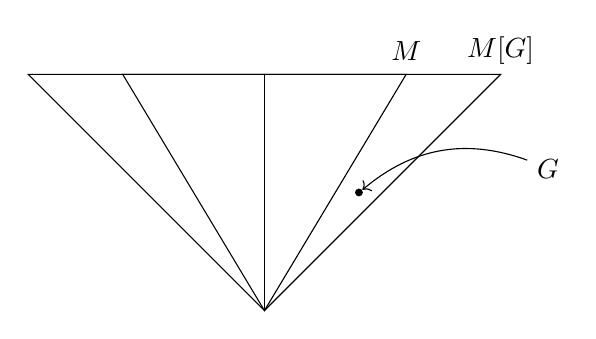
\begin{tikzpicture}[scale=3]
    \draw (0,0) -- (0.6,1) -- (-0.6,1) -- cycle;
    \draw (0,0) -- (1,1) -- (-1,1) -- cycle;
    \draw (0,0) -- (0,1);
    \node [dot] (dot) at (0.4,0.5) {};
    \node at (0.6,1.1) {$M$};
    \node at (1,1.1) {$M[G]$};
    \node (G) at (1.2,0.6) {$G$};
    \draw [->] (G) to[bend right] (dot);
  \end{tikzpicture}
\end{center}
% powerset discussion
It would be nice to be able to talk about whether a name $\sigma$ is a name for a subset of $\val(\tau,G)$ without referring to the precise set-theoretic make-up of $\tau$ and $\sigma$.

\begin{defi}
  \hypertarget{def:lmp}The \named{forcing language}, written $\mathcal{L}(M^\mathbb{P})$, is just $\mathcal{L}_\in$ augmented with one constant symbol for each $\tau \in M^{\mathbb{P}}$.
  If $G$ is $\mathbb{P}$-generic over $M$, there is a canonical interpretation of $\mathcal{L}(M^\mathbb{P})$ in $M[G]$.
  \begin{align*}
    M[G] \models \varphi(\tau_1, \dotsc, \tau_n) :\Longleftrightarrow M[G] \models \varphi(\val(\tau_1,G),\dotsc,\val(\tau_n,G)).
  \end{align*}
  \hypertarget{def:forcingrelation}If $\varphi$ is a sentence of $\mathcal{L}(M^{\mathbb{P}})$ and $p \in \mathbb{P}$, the \named{forcing relation} is
  \begin{align*}
    p \Vdash_M \varphi :\Longleftrightarrow \text{for every } \mathbb{P}\text{-generic filter $G$ over $M$ such that $p \in G$, we have $M[G] \models \varphi$}.
  \end{align*}
\end{defi}
\subsection{Forcing relations}
We will eventually prove:
\begin{thm}[Forcing theorem]
  The following are equivalent:
  \begin{enumerate}
  \item $M[G] \models \varphi$
  \item $\exists p \in G \ (M \models p \Vdash \varphi)$.
  \end{enumerate}
\end{thm}
\begin{thm}
  The \hyperlink{def:forcingrelation}{forcing relation} is definable in $M$:
  there is a definable relation $p \Vdash^* \varphi$ such that
  \begin{equation*}
    \forall p, \varphi \quad p \Vdash \varphi \iff p \Vdash^* \varphi.
  \end{equation*}
\end{thm}
\newlec
Technically, the meaning of $\hyperlink{def:mg}{M[G]} \models \varphi$ does not just depend on $M[G]$, but on $G$ itself, from the definition above.
Better notation would look like $M[G],G \models \varphi$.

Similarly, we should more precisely write $\Vdash_M$ for the forcing relation.
A priori, $\Vdash$ is not definable in $M$, but we'll show that it is.
We shall give a different definition of a relation $p \Vdash^* \varphi$ which is definable in $M$ and show $p \Vdash ^* \varphi$ iff $p \Vdash \varphi$.
We call $\Vdash^*$ the \named{syntactic forcing relation}\index{forcing relation!syntactic} and $\Vdash$ the \named{semantic forcing relation}\index{forcing relation!semantic}.

Let's restate the forcing theorem more formally.
\begin{thm}[Forcing theorem]\hypertarget{thm:forcing}
  Let $M$ be a countable \hyperlink{def:transitive}{transitive} model of \hyperlink{def:axioms}{set theory} and $\mathbb{P} \in M$.
  Let $\varphi$ be a sentence in the \hyperlink{def:lmp}{forcing language}.
  Then the following are equivalent.
  \begin{enumerate}[(i)]
    \item $\hyperlink{def:mg}{M[G]} \models \varphi$
    \item there is a $p \in G$ such that $M \models p \Vdash^* \varphi$
  \end{enumerate}
\end{thm}
(Note that we haven't defined $\Vdash^*$ yet).
Let's prove the equivalence of $\Vdash^*$ and $\Vdash$ from the \hyperlink{thm:forcing}{Forcing theorem}.
\begin{prop}
  Let $M$ be countable \hyperlink{def:transitive}{transitive} model, $\mathbb{P} \in M$, $p \in \p$, $\varphi$ a sentence of \hyperlink{def:lmp}{$\mathcal{L}(M^{\p})$}.
\end{prop}
\begin{proof}
  Suppose $p \Vdash_M \varphi$. For every $G$ which is \hyperlink{def:genericO}{$\mathbb{P}$-generic over $M$} with $p \in G$, $M[G] \models \varphi$.
  By the \hyperlink{thm:forcing}{Forcing theorem}, find $q \in G$ such that $M \models q \Vdash^* \varphi$.

  Closure properties of \hyperlink{def:forcingrelation}{$\Vdash$}:
  \begin{enumerate}
    \item If $p \Vdash \varphi$ and $q \leq p$ then $q \Vdash \varphi$.
    \item If $p \Vdash \varphi$ and $p \Vdash \psi$, then $p \Vdash \varphi \land \psi$.
  \end{enumerate}
  We know that $p,q \in G$, so there is some $r \in G$ such that $r \leq p,q$. By 1, we get that $r \Vdash \varphi$.
  Stuck...
\end{proof}
Let's postpone this until we have actually defined $\Vdash^*$.
\begin{defi}\hypertarget{def:densebelow}
  We say that $D$ is \textbf{dense below} $p$ if
  \begin{equation*}
    \forall q \leq p \ \exists r \leq q \ r \in D.
  \end{equation*}
\end{defi}
\begin{defi}
  \hypertarget{def:syn}Now we define $\Vdash^*$ by recursion on the rank of the names involved and the complexity of $\varphi$.
  It suffices to:
  \begin{enumerate}
    \item define for $\tau_1 \in \tau_2$ where $\tau_1,\tau_2$ are names.
    \item define for $\tau_1 = \tau_2$ where $\tau_1,\tau_2$ are names.
    \item conjunctions: from $\varphi,\psi$ define for $\varphi \land \psi$.
    \item negation: from $\varphi$ define for $\neg\varphi$.
    \item existential: from $\varphi$ define for $\exists x\ \varphi$.
  \end{enumerate}
  In particular, we set
  \begin{enumerate}
    \setcounter{enumi}{2}
    \item $p \Vdash^* \varphi \land \psi$ iff $p \Vdash^* \varphi$ and $p \Vdash^* \psi$. (Remark: We have no choice here due to property 2 in the failed proof).
    \item $p \Vdash^* \neg \varphi$ iff $\forall q \leq p$, $p \not\Vdash^* \varphi$.
    \item $p \Vdash^* \exists x\ \varphi(x, \tau_1, \dotsc, \tau_n)$ iff
      \begin{align*}
      \{r \mid \text{there is a }\p\text{-}\hyperlink{def:name}{\text{name }}\sigma\text{ such that } r \Vdash^* \varphi(\sigma,\tau_1, \dotsc, \tau_n)\}
      \end{align*}
      is \hyperlink{def:densebelow}{dense below} $p$.
    \setcounter{enumi}{0}
    \item $p \Vdash^* \tau_1 \in \tau_2$ iff
      \begin{align*}
        \{q \mid \text{there is $(\pi,s) \in \tau_2$ such that $q \leq s$ and } q \Vdash^* \pi = \tau_1\}
      \end{align*}
      is dense below $p$.
    \item $p \Vdash^* \tau_1 = \tau_2$ iff for all $(\pi_1, s_1) \in \tau_1$,
      \begin{align*}
        \{q \mid q \leq s_1 \rightarrow \exists (\pi_2,s_2) \in \tau_2\text{ such that }q \leq s_2\text { and }q \Vdash^* \pi_1 = \pi_2\}
      \end{align*}
      is dense below $p$ and for all $(\pi_2, s_2) \in \tau_2$,
      \begin{align*}
        \{q \mid q \leq s_2 \rightarrow \exists (\pi_1,s_1) \in \tau_1\text{ such that }q \leq s_1\text{ and }q \Vdash^* \pi_1 = \pi_2\}
      \end{align*}
      is dense below $p$.
  \end{enumerate}
\end{defi}
Note that only 5 is not absolute.

\newlec
From Example Sheet 3, exercise 23, we have:
\begin{enumerate}[(1)]
  \item If $D$ is \hyperlink{def:densebelow}{dense below} $p$ and $r \leq p$, then $D$ is dense below $r$.
  \item If $\{r \mid D \text{ is dense below }r\}$ is dense below $p$, then $D$ is dense below $p$.
\end{enumerate}
\begin{lemma}\hypertarget{lem:forc}
  The following are equivalent:
  \begin{enumerate}[(i)]
    \item $p \hyperlink{def:syn}{\Vdash^*} \varphi$
    \item $\forall r \leq p \ (r \Vdash^* \varphi)$
    \item $\{r \mid r \Vdash^* \varphi\}$ is \hyperlink{def:densebelow}{dense below} $p$.
  \end{enumerate}
\end{lemma}
\begin{proof}
  Clearly (ii) $\Rightarrow$ (i), (iii).
  Let's show (i) $\Rightarrow$ (ii). Proof by induction on the \hyperlink{def:syn}{definition of $\Vdash^*$}.
  Of the five parts of the recursion, 1,2,5 are formulated in terms of `\hyperlink{def:densebelow}{dense below $p$}':
  \begin{equation*}
    p \Vdash^* \varphi \iff X_\varphi \text{ is dense below } p
  \end{equation*}
  By Exercise 23 as quoted above, if $r \leq p$ and $X_\varphi$ is dense below $p$, $X_\varphi$ is dense below $r$. Observe that cases 3 and 4 of (i) $\Rightarrow$ (ii) follow directly from definition.

  Similarly, (iii) $\Rightarrow$ (i) goes by recursion via 1.-5.\ using item (2) of the exercise rather than item (1).
\end{proof}
\begin{cor}
  \begin{equation*}
  p \hyperlink{def:forcingrelation}{\forces_M} \varphi \iff M \models p \hyperlink{def:syn}{\forces^*} \varphi.
  \end{equation*}
  (assuming the \hyperlink{thm:forcing}{forcing theorem} and the \hyperlink{lem:forc}{lemma}).
\end{cor}
\begin{proof}
  Assume $p \hyperlink{def:forcingrelation}{\forces_M} \varphi$.
  So for any $G$ such that $p \in G$, $\hyperlink{def:mg}{M[G] \models} \varphi$.
  The \hyperlink{thm:forcing}{Forcing Theorem} says $\exists q \in G$ such that $M \models q \hyperlink{def:syn}{\forces^*} \varphi$.
  We want to show $p \Vdash^* \varphi$.
  By the \hyperlink{lem:forc}{lemma}, it's enough to show
  \begin{align*}
    D \coloneqq \{r \mid r \forces^* \varphi\} \text{ is \hyperlink{def:densebelow}{dense below} } p
  \end{align*}

  Fix any $q' \leq p$.
  Since $M$ is a countable \hyperlink{def:transitive}{transitive} model of \hyperlink{def:axioms}{\textsf{ZFC}}, there is some $H$ with $q' \in H$ and $H$ is $\mathbb{P}$-\hyperlink{def:genericO}{generic over $M$}.
  Since $q' \leq p$, we know $p \in H$.
  So by $p \forces_M \varphi$, we get $M[H] \models \varphi$.
  Apply the Forcing Theorem here and get $q'' \in H$ such that $M \models q'' \forces^* \varphi$.
  But then $q'' \in D \cap H$. Since $H$ is a filter, we find $r \leq q', q''$ with $r \in H$.
  $r$ witnesses that $D$ is dense below $p$.

  Now assume $M \models p \forces^* \varphi$.
  Want to show $p \forces_M \varphi$.
  Let $G$ be $\mathbb{P}$-generic over $M$ with $p \in G$. By the Forcing Theorem, $M[G] \models \varphi$, as required.
\end{proof}

\subsection{Proving the Forcing Theorem}
It still remains to prove the \hyperlink{thm:forcing}{Forcing Theorem}.
\begin{proof}[Proof of \hyperlink{thm:forcing}{Forcing Theorem}]
  We'll prove this by induction
  \begin{enumerate}[(a)]
    \item rank of names
    \item assume that $=$ is done
    \item[(c)-(e)] complexity of formulas.
  \end{enumerate}
  We'll do this in the order 3,4,5,1,2 (increasing difficulty).
  Induction statement:
  \begin{equation*}
    \hyperlink{def:mg}{M[G] \models} \varphi \iff \exists p \in G, \ M \models p \hyperlink{def:syn}{\Vdash^*} \varphi.
  \end{equation*}
  \begin{enumerate}\setcounter{enumi}{2}
    \item
      Assume the induction hypothesis holds for $\varphi$ and $\psi$.

      ($\Rightarrow$)
      \begin{align*}
        M[G] \models \varphi \land \psi &\Rightarrow M[G]  \models \varphi \text{ and } M[G] \models \psi \\
                                        &\Rightarrow \exists p \in G \ p \Vdash^* \varphi \text{ and } \exists q \in G \ q \Vdash^* \psi \\
                                        &\Rightarrow \exists r \leq p,q,\ r \in G \text{ so by Lemma } r \Vdash^* \varphi \text{ and } r \Vdash^* \psi \\
                                        &\Rightarrow \exists r \in G\ r \Vdash^* \varphi \land \psi.
      \end{align*}
      by definition.

      ($\Leftarrow$) Assume $p \in G$
      \begin{align*}
        p \forces^* \varphi \land \psi &\Rightarrow p \forces^* \varphi \text{ and } p \Vdash^* \psi \\
                                       &\Rightarrow M[G] \forces \varphi \text{ and } M[G] \forces \psi \\
                                       &\Rightarrow M[G] \forces \varphi \land \psi.
      \end{align*}
    \item ($\Rightarrow$) We are now considering $M[G] \models \neg\varphi$, using the induction hypothesis for $\varphi$. Consider
      \begin{align*}
        \mathcal{D} \coloneqq \{p \mid p \forces^* \varphi \text{ or } p \forces^* \neg \varphi \}.
      \end{align*}
      Claim: $\mathcal{D}$ is \hyperlink{def:dense}{dense}. Proof: Obvious from definition of \hyperlink{def:syn}{syntactic forcing} of negation 4.

      Thus find $p \in \mathcal{D} \cap G$. If $p \forces^* \neg \varphi$, done.
      Suppose $p \Vdash^* \varphi$. Then by induction hypothesis, $M[G] \models \varphi$. Contradiction!

      ($\Leftarrow$) Now assume $p \in G$ and $p \forces^* \neg \varphi$. Suppose $M[G] \models \varphi$ for contradiction.
      By the induction hypothesis, find $q \in G$ with $q \forces^* \varphi$. Find $r \leq p,q$ with $r \in G$.
      By the \hyperlink{lem:forc}{Lemma}, $r \forces^* \varphi$ but by definition of $p \forces^* \neg \varphi$, $r \not\forces^* \varphi$. Contradiction.

    \item[5.] ($\Rightarrow$) We have $M[G] \models \exists x \ \varphi(x)$. But $\varphi(x)$ is not a sentence, so isn't part of the induction hypothesis. Instead, the induction hypothesis works for $\varphi(\sigma / x)$ for any $\sigma \in M^{\mathbb{P}}$.
      \begin{align*}
        &\Rightarrow \text{there is } a \in M[G] \ M[G] \models \varphi(a / x) \\
        &\Rightarrow \text{there is } \sigma \in M^\mathbb{P} \ M[G] \models \varphi(\sigma / x) \\
        &\Rightarrow \text{there is } p \in G \text{ such that } M \models p \forces^* \varphi(\sigma / x)
        \intertext{Thus $\{r \mid \text{there is } \sigma \text{ with } \sigma \forces^* \varphi(\sigma/x)\}$ is not only \hyperlink{def:densebelow}{dense below} $P$, but is everything below $p$.}
        &\Rightarrow p \forces^* \exists x\ \varphi.
      \end{align*}

      ($\Leftarrow$) Conversely, assume $p \in G$ with $p \forces^* \exists x \; \varphi$.
      By definition,
      \begin{align*}
        \mathcal{D} \coloneqq \{r \mid \text{there is } \sigma \text{ with } r \forces^* \varphi(\sigma/x)\}
      \end{align*}
      is dense below $p$. Find $r \in \mathcal{D}  \cap G$.
      Fix a witness $\sigma$ to the fact that $r \in \mathcal{D}$,
      so $r \forces^* \varphi(\sigma/x)$.
      By the induction hypothesis,
      \begin{align*}
        M[G] &\models \varphi(\sigma/x) \\
        M[G] &\models \varphi(\val(\sigma,G)/x) \text{ so } M[G] \models \varphi(a/x) \text{ where } a = \val(\sigma,G)
      \end{align*}
      So: $M[G] \models \exists x \ \varphi$.

    \item[1.] $(\Leftarrow)$ Let $p \in G$ such that $p \forces^* \tau_1 \in \tau_2$.
      Induction hypothesis only applies for $=$ now.
      By definition
      \begin{align*}
        \mathcal{D} \coloneqq \{q \mid \exists (\pi,s) \in \tau_2 \ (q \leq s \land q\forces^* \pi = \tau_1)\}
      \end{align*}
      is dense below $p$, so
      find $q \in \mathcal{D} \cap G$.
      Fix $(\pi,s) \in \tau_2$ such that
      \begin{align*}
        q \leq s \quad \text{and} \quad q \forces^* \pi = \tau_1.
      \end{align*}
      This gives $s \in G$, so $\val(\pi,G) \in \val(\tau_2,G)$.
      By the induction hypothesis, we also get $M[G] \models \pi = \tau_1$, i.e.\ $\val(\pi,G) = \val(\tau_1, G)$.
      This gives $\val(\tau_1,G) \in \val(\tau_2,G)$, so $M[G] \models \tau_1 \in \tau_2$.

      \newlec
      ($\Rightarrow$) We have $M[G] \models \tau_1 \in \tau_2$, thus $\val(\tau_1, G) \in \val(\tau_2,G)$.
      Note this doesn't give $\tau_1 \in \tau_2$ as names, only that there is some $(\pi,s) \in \tau_2$ with $s \in G$ and $\val(\pi,G) = \val(\tau_1,G)$.
      This means $M[G] \models \pi = \tau_1$, so by the induction hypothesis find $r \in G$ with $r \forces^* \pi = \tau_1$.
      Find $p \leq s,r$ with $p \in G$. Then
      \begin{align*}
        \{q \leq p \mid \exists(\bar{\pi}, \bar{s}) \in \tau_2 \ (q \leq \bar{s} \land q \forces^* \bar{\pi} = r_1)\}
      \end{align*}
      This set, or even the smaller set
      \begin{align*}
        \{q \leq p \mid q \leq s \land q \forces^* \pi = r_1\}
      \end{align*}
      is everything below $p$, thus \hyperlink{def:dense}{dense}.

    \item[2.] $(\Leftarrow)$ Fix $p \in G$ such that $p \forces^* \tau_1 = \tau_2$. Our induction hypothesis now only applies to $=$ with names of lower rank.
      The form of the definition of $p \forces^* \tau_1 = \tau_2$ is symmetric in the sense that if we're using the first half to show that $\val(\tau_1, G) \subseteq \val(\tau_2,G)$, then the other half shows $\val(\tau_2,G) \subseteq \val(\tau_1,G)$.

      So, we'll show $\val(\tau_1,G) \subseteq \val(\tau_2,G)$.
      Fix $x \in \val(\tau_1,G)$.
      Fix a $(\pi_1,s_1) \in \tau_1$ such that $s_1 \in G$ and $\val(\pi_1,G) = x$.
      Since $G$ is a filter, find $r \leq p,s_1$ with $r \in G$.
      \begin{align*}
        \mathcal{D} \coloneqq \{ q \leq r \mid q \leq s_1 \Rightarrow \exists(\pi_2, s_2) \in \tau_2 \ (q \leq s_1 \land q \forces^* \pi_1=\pi_2)\}
      \end{align*}
      is dense below $r$.
      Find $q \in \mathcal{D} \cap G$. Since $r \leq s_1$, we know that $q \leq r \leq s_1$, so the antecedent in the definition of $\mathcal{D}$ is true, so there is $(\pi_2,s_2) \in \tau_2$ with $q \leq s_2 \land q \forces^* \pi_1 = \pi_2$.

      As earlier, we get $s_2 \in G$, thus $\val(\tau_2,G) \in \val(\tau_2,G)$. $\pi_1 \in \tau_1$ and $\pi_2 \in \tau_2$, so both have lower rank, thus by the induction hypothesis, $M[G] \models \pi_1 = \pi_2$, i.e.\ $\val(\pi_1,G) = \val(\pi_2,G)$.
      Hence, $x=\val(\pi_1,G) \in \val(\tau_2,G)$.

      $(\Rightarrow)$ Assume $M[G] \models \tau_1 = \tau_2$, that is $\val(\tau_1,G) = \val(\tau_2,G)$,
      Consider
      \begin{align*}
        \mathcal{D}_1 &\coloneqq \{r \mid r \forces^* \tau_1 = \tau_2\}\\
        \mathcal{D}_2 &\coloneqq \left\{r\ \middle\vert\
          \begin{gathered}
            \text{there is } (\pi_1,s_1) \in \tau_1 \ \big(r \leq s_1 \text{ and for all }(\pi_2,s_2) \in \tau_2\\ \text{and all } q \ ((q \leq s_2 \land q \forces^* \pi_1 = \pi_2) \rightarrow q \hyperlink{def:incompat}{\perp} r)\big)
          \end{gathered}
        \right\}\\
        \mathcal{D}_3 &\coloneqq \left\{r\ \middle\vert\
            \begin{gathered}
              \text{there is } (\pi_2,s_2) \in \tau_2 \ \big(r \leq s_2 \text{ and for all }(\pi_1,s_1) \in \tau_1\\ \text{and all } q \ ((q \leq s_1 \land q \forces^* \pi_1 = \pi_2) \rightarrow q \perp r)\big)
            \end{gathered}
          \right\}\\
        \mathcal{D} &\coloneqq \mathcal{D}_1 \cup \mathcal{D}_2 \cup \mathcal{D}_3
      \end{align*}

      \begin{observation}
        If $r \in G$, then neither $r \in \mathcal{D}_2$ nor $r \in \mathcal{D}_3$ can hold. By symmetry, it's enough to deal with $ \mathcal{D}_2$ .
        Towards a contradiction, assume $r \in G$ and $r \in \mathcal{D}_2$.

        Find $(\pi,s_1) \in \tau_1$ with desired properties.
        Since $r \leq s_1 \Rightarrow s_1 \in G$ so
        \begin{align*}
          \val(\pi_1, G) \in \val(\tau_1,G) = \val(\tau_2,G).
        \end{align*}
        So there is $(\pi_2,s_2) \in \tau_2$ with $s_2 \in G$ and $\val(\pi_2,G) = \val(\pi_1, G)$.
        By induction hypothesis, find $q' \in G$ with $q' \forces^* \pi_1 = \pi_2$.
        Find $q \leq r,s_1,s_2, q'$ so $q$ contradicts $r \in \mathcal{D}_2$, as required.
      \end{observation}

      So, we're done if we show that $\mathcal{D}$ is dense.
      Fix $p \in \p$. If $p \forces^* \tau_1 = \tau_2$, then $p \in \mathcal{D}$ done.
      If it doesn't, we'll find $r \leq p$ for $p \in \mathcal{D}_2$ or $\mathcal{D}_3$.
      Again by symmetry, we'll show: If the first half of the definition of $p \not\forces^* \tau_1 = \tau_2$ fails, then find $r \in \mathcal{D}_2 $.

      \newlec
      We showed if $p \in G$ then neither $p \in \mathcal{D}_2$ or $p \in \mathcal{D}_3$ can hold. Thus if $p \in G \cap \mathcal{D} $ then $p \forces^* \tau_1 = \tau_2$.
      So: need to show that $ \mathcal{D} $ is dense.
      Let $p \in \p$ be arbitrary. If $p \forces^* \tau_1 = \tau_2$, done. So assume $p \not\forces^* \tau_1 = \tau_2$.

      We will show that if the first half of the definition of $ p\forces^* \tau_1 = \tau_2$ is violated, then we find $r \leq p$ such that $r \in \mathcal{D} _2$. (Similarly, if the second half is violated, then for some $r \leq p$, we have $r \in \mathcal{D} _3$)
      The first half fails means:
      there is $(\pi_1,s_1) \in \tau_1$ such that
      \begin{equation*}
        \mathcal{D}' \coloneqq \{p \leq p \mid q \leq s_1 \rightarrow \exists (\pi_2,s_2) \in \tau_2 \ (q \leq s_2 \land q \forces^* \pi_1 = \pi_2)\}
      \end{equation*}
      is not dense below $p$.
      Fix this $(\pi_1, s_1) \in \tau_1$ and fix $r \leq p$ such that $\mathcal{D}'$ has no element below $r$.
      That is,
      \begin{equation*}
        \forall q \leq r \ (q \leq s_1 \land \forall (\pi_2,s_2) \in \tau_2 \ (q \nleq s_2 \lor q \not\forces^* \pi_1 = \pi_2)) \tag{$*$}\label{eq:1}
      \end{equation*}

      Fix arbitrary $(\pi_2,s_2) \in \tau_2$ and $q$ such that
      \begin{equation*}
        q \leq s_2 \land q \forces^* \pi_1 = \pi_2 \tag{$**$} \label{eq:2}
      \end{equation*}
      If $q$ is compatible with $r$, find $q' \leq r,q$ satisfying \eqref{eq:1}.
      But now $q' \not\forces^* \pi_1 = \pi_2$ by \eqref{eq:1} and $q' \forces^* \pi_1 = \pi_2$ by \eqref{eq:2} and $q' \leq q$.
      Contradiction.
      So $q \perp r$, as required. \qedhere
  \end{enumerate}
\end{proof}

\begin{thm}[Generic Model Theorem]\hypertarget{thm:genericmodel}
  Take $M$ a countable \hyperlink{def:transitive}{transitive} model of \hyperlink{def:axioms}{\textsf{ZFC}}, $\mathbb{P} \in M$, and say $G$ is $\mathbb{P}$-\hyperlink{def:genericO}{generic over} $M$,
  \begin{equation*}
    \hyperlink{def:mg}{M[G]} \models \textsf{ZFC}.
  \end{equation*}
\end{thm}
\begin{cor}
  \hyperlink{def:mg}{$M[G]$} is the minimal \hyperlink{def:transitive}{transitive} model of \hyperlink{def:axioms}{\textsf{ZFC}} with $M \subseteq M[G]$, $G \in M[G]$.
\end{cor}
Observe that if $M = \hyperlink{def:l}{L_\alpha}$ for some countable $\alpha$ and $L_\alpha(G)$ is the relativised $L$-construction as on Example Sheet 2, then by \hyperlink{thm:min}{minimality} of $L$ (or $L(G)$ for models containing $G$), $M[G] = L_\alpha(G)$.

\begin{proof}[Proof of \hyperlink{thm:genericmodel}{Generic Model Theorem}]\leavevmode
  \begin{description}
    \item[\textsf{Ext}] Follows by \hyperlink{def:transitive}{transitivity} of \hyperlink{def:mg}{$M[G]$}
    \item[\textsf{Found}] Follows by transitivity of $M[G]$
    \item[\textsf{Pair}] Was proved \hyperlink{prop:mgpair}{earlier} by hand
    \item[\textsf{Union}] On Example Sheet 3, by hand
    \item[\textsf{Inf}] By absoluteness of `$x = \mathbb{N}$', we only need $\mathbb{N} \in M[G]$.
      But $\mathbb{N} = \hyperlink{def:val}{\val}(\check{\mathbb{N}},G)$
    \item[\textsf{Choice}] On Example Sheet 4
    \item[\textsf{Repl}] On Example Sheet 4
    \item[\textsf{Sep}] Fix a formula $\varphi$, parameters $x_1, \dotsc, x_n \in \hyperlink{def:mg}{M[G]}$ and $x \in M[G]$. We would like to construct
      \begin{align*}
        \{z \in x \mid M[G] \models \varphi(z, x_1, \dotsc, x_n)\}.
      \end{align*}
      Fix names $\tau_1, \dotsc, \tau_n$ for $x_1, \dotsc, x_n$, and $\sigma$ for $x$.
      Set
      \begin{align*}
        A &\coloneqq \{z \in \hyperlink{def:val}{\val}(\sigma,G) \mid M[G] \models \varphi(z, \tau_1, \dotsc, \tau_n)\} \\
        \rho &\coloneqq \{(\pi,p) \mid p \hyperlink{def:syn}{\forces^*} \pi \in \sigma \land \varphi(\pi, \tau_1, \dotsc, \tau_n)\}
      \end{align*}
      Claim: $A = \hyperlink{def:val}{\val(\rho,G)}$.

      ($\supseteq$) Suppose $z \in \val(\rho,G)$. There is $(\pi,p) \in \rho$ with $p \in G$ and $\val(\pi,G) = z$.
      $(\pi,p) \in \rho$ means that
      \begin{align*}
        p \forces^* \pi \in \sigma \land \varphi(\pi, \tau_1, \dotsc, \tau_n)
      \end{align*}
      By the \hyperlink{thm:forcing}{Forcing Theorem}, $M[G] \models \pi \in \sigma \land \varphi(\pi, \tau_1, \dotsc, \tau_n)$.
      Thus $M[G] \models z \in x \land \varphi(z, x_1, \dotsc, x_n)$
      so $z \in A$.

      ($\subseteq$) Let $z \in A$, so $z \in x$ and $M[G] \models \varphi(z, x_1, \dotsc, x_n)$. Fix $\pi$ name for $z$: $z=\val(\pi,G)$.
      The Forcing Theorem together with $z \in x$ says there is $p \in G$  with $p \forces^* \pi \in \sigma$.
      Similarly, the Forcing Theorem together with $M[G] \models \varphi(z, x_1, \dotsc, x_n)$ gives that there is $q \in G$ with $q \forces^* \varphi(\pi, \tau_1, \dotsc, \tau_n)$.
      Find $r \leq p,q$ with $r \in G$.
      Then $r \models^* \pi \in \sigma \land \varphi(\pi, \tau_1, \dotsc, \tau_n)$. So by definition, $(\pi,r) \in \rho$.
      $z = \val(\pi,G) \in \val(\rho,G)$.
    \item[\textsf{Pow}] Since we have Separation, it's enough to show
      \begin{equation*}
        \forall x\ \exists y\ \forall z\ (z \subseteq x \rightarrow z \in y).
      \end{equation*}
      Fix a name $\sigma$ for $x$. Let's write for any name $\tau$:
      \begin{align*}
        \dom(\tau) \coloneqq \{\tau' \mid \exists (\tau',p) \in \tau\}
      \end{align*}
      We think of names for subsets of $x$ as names whose domain is a subset of the domain of $\sigma$.
      \begin{align*}
        \rho_\sigma \coloneqq \{(\tau,\1) \mid \dom(\tau) \subseteq \dom(\sigma)\}
      \end{align*}
      Let's prove that $\val(\rho_\sigma,G)$ satisfies $\forall z \ (z \subseteq x \rightarrow z \in \val(\rho_\sigma,G))$.
      Assume that $z \subseteq x$. Fix a name $\mu$ for $z$: $\val(\mu,G) = z$.
      Define
      \begin{equation*}
        \mu^* \coloneqq \{(\pi,p) \mid \pi \in \dom(\sigma) \text{ and } p \forces^* \pi \in \mu\}.
      \end{equation*}
      By def, $\dom(\mu^*) \subseteq \dom(\sigma)$. So $(\mu^*,\1) \in \rho_\sigma$. Hence $\val(\mu,G) \in \val(\rho_\sigma,G)$.
      Remains to show $\val(\mu,G) = \val(\mu^*,G)$.

      If $w \in \val(\mu,G)$: Since $\val(\mu,G) \subseteq \val(\sigma,G)$, we find $(\pi,p) \in \sigma$ with $p \in G$ such that $\val(\pi,G) = w$.
      $M[G] \models \pi \in \mu$. By the Forcing Theorem, there is $q \in G$ with $q \forces^* \pi \in \mu$.
      So $(\pi,q) \in \mu^*$. Since $q \in G$, this means $\val(\pi,G) \in \val(\mu^*,G)$.

      If $w \in \val(\mu^*,G)$, find $(\pi,p) \in \mu^*$, $p \in G$ with $w = \val(\pi,G)$. By definition, $p \forces^* \pi \in \mu$.
      The Forcing Theorem says $M[G] \models \pi \in \mu$, thus $w = \val(\pi,G) \in \val(\mu,G)$. \qedhere
  \end{description}
\end{proof}

\subsection{Consistency proofs}
\newlec
We will show that \hyperlink{def:vl}{\textsf{V$\neq$L}} is consistent.
Suppose $M$ is a countable \hyperlink{def:transitive}{transitive} model of \hyperlink{def:axioms}{\textsf{ZFC}} + \textsf{V=L}.
By our work on $L$, we know that there is $\alpha < \omega_1$ such that $M = \hyperlink{def:l}{L_\alpha}$.
Let $\mathbb{P} \in L_\alpha$ be any partial order that is \hyperlink{def:splitting}{splitting}.
By countability, we get a $G$ which is \hyperlink{def:genericO}{$\p$-generic over $M$}, and $G \notin M$ by splitting.
So $\hyperlink{def:mg}{M[G]} \neq M$.

Claim: $M[G] \models \textsf{V$\neq$L}$. Suppose not, then $M[G] = L_\beta$ for some $\beta$. Then $\text{Ord} \cap M[G] = \text{Ord} \cap M = \alpha$.
So $\beta = \alpha$. So $M[G] = L_\beta = L_\alpha = M$, a contradiction.

Note this didn't use any property of $\p$, other than that it is splitting.
We might be able to do more if we use specific $\p$s.
So, let's remind ourselves of the specific $\p$s we have:
\begin{align*}
  \p &= \operatorname{Fn}(X,Y) \quad \text{where } X,Y \in M \\
     &= \{ p \mid p \text{ is a partial function from } X \text{ to } Y \text{ with finite domain}\}.
\end{align*}
If $G$ is $\mathbb{P}$-generic over $M$, then $\bigcup G \eqqcolon f_G: X \to Y$ surjective.
So if $X = \mathbb{N}$, then $M[G] \models Y$ is countable.
In particular, if $Y = \aleph_1^M$, then forcing with $\operatorname{Fn}(\mathbb{N},\aleph_1^M)$ will `collapse' $\aleph_1^M$:
\begin{align*}
  M[G] \models \aleph_1^M \text{ is a countable ordinal.}
\end{align*}

\textbf{Excursion.} Suppose $M \models 2^{\aleph_0} = \aleph_2$ and $\mathbb{P} = \operatorname{Fn}(\mathbb{N},\aleph_1^M)$.
If $\aleph_1^M$ is no longer a cardinal in $\hyperlink{def:mg}{M[G]}$, then the original bijection $f: \mathbb{R}^M \to \aleph_2^M$ will be a bijection between $\mathbb{R}^M$ and an ordinal which can be at best $\aleph_1^{M[G]}$.
In order to make this into a proof of $M[G] \models \textsf{CH}$, we need:
\begin{enumerate}
  \item $M[G] \models \aleph_2^M$ is a cardinal, thus $M[G] \models \aleph_2^M = \aleph_1$.
  \item $M[G] \models |\mathbb{R}| = |\mathbb{R}^M|$
\end{enumerate}
Since $\aleph_1^M < \aleph_1^{M[G]}$, we know $\mathbb{R}^{M[G]} \supsetneqq \mathbb{R}^M$.
If we had 1 and 2, we get a consistency proof of \textsf{ZFC} + \textsf{CH} + \textsf{V$\neq$L}.

\medskip
Back to forcing $\neg$\textsf{CH}.
Instead, take $\p \coloneqq \text{Fn}(\mathbb{N} \times \aleph_2^M, \mathbb{N})$.
This generates
\begin{equation*}f_G = \bigcup G: \mathbb{N} \times \aleph_2^M \to \mathbb{N}.\end{equation*}
Define in $M[G]$ for $\alpha < \aleph_2^M$:
\begin{align*}
  f_\alpha(n) &\coloneqq f(n,\alpha) \\
  f_\alpha&: \mathbb{N} \to \mathbb{N}.
\end{align*}
We'll show that if $\alpha \neq \beta$ then $f_\alpha \neq f_\beta$.
In particular, the map
\begin{align*}
  \alpha \mapsto f_\alpha
\end{align*}
gives an injection from $\aleph_2^M$ into $\mathbb{N}^\mathbb{N}$.
Then $\hyperlink{def:mg}{M[G]} \models |\aleph_2^M| \leq 2^{\aleph_0}$.

\begin{proof}[Proof of injectivity]
  Fix $\alpha \neq \beta$ and define
  \begin{align*}
    D_{\alpha,\beta} \coloneqq \{p \mid \exists n \ p(n,\alpha) \neq p(n,\beta)\}.
  \end{align*}
  I claim $D_{\alpha,\beta}$ is dense. Fix $p \in \p$ arbitrarily. Then $\dom(p)$ is finite, so find $m \in \mathbb{N}$ such that both $(n,\alpha), (n,\beta) \notin \dom(p)$
  \begin{align*}
    q \coloneqq p \cup \{((n,\alpha), 0), ((n,\beta),1)\}
  \end{align*}
  So $q(n,\alpha) \neq q(n,\beta)$, so $q \leq p$, $q \in D_{\alpha,\beta}$.
  Find $p \in G \cap D_{\alpha,\beta}$. Then $f_G = \bigcup G$ with $p \in G$, so there is $n$ such that
  \begin{align*}
    f_G(n,\alpha) &\neq f_G(n,\beta) \\
    \Rightarrow f_\alpha(n) &\neq f_\beta(n) \\
    \Rightarrow f_\alpha &\neq f_\beta. \qedhere
  \end{align*}
\end{proof}
So to summarise, if $G$ is $\operatorname{Fn}(\mathbb{N} \times \aleph_2^M, \mathbb{N})$-\hyperlink{def:genericO}{generic} over $M$, then
\begin{align*}
  \hyperlink{def:mg}{M[G]} \models 2^{\aleph_0} \geq |\aleph_2^M|
\end{align*}
We need therefore:
\begin{align*}
  \aleph_1^M &= \aleph_1^{M[G]} \\
  \aleph_2^M &= \aleph_2^{M[G]}
\end{align*}
in order to get $M[G] \models 2^{\aleph_0} \geq \aleph_2$.
\begin{defi}\hypertarget{def:pcard}
  Let $M$ a countable \hyperlink{def:transitive}{transitive} model, and $\p \in M$.
  We say that $\p$ \named{preserves cardinals} if for all $\alpha$ an ordinal and all $G$ which is $\p$-generic over $M$, we have
  \begin{align*}
    M \models \alpha \text{ is a cardinal} \iff M[G] \models \alpha \text{ is a cardinal}.
  \end{align*}
  Note $\Leftarrow$ follows from the fact that `is a cardinal' is \hyperlink{def:pi1}{$\Pi_1$}.
\end{defi}

\begin{thm}
  If $M \models \p$ has the \hyperlink{def:ccc}{countable chain condition}, then $\p$ \hyperlink{def:pcard}{preserves cardinals}.
\end{thm}

Putting this all together, from sheet 3 we know that if $Y$ is countable, then $\operatorname{Fn}(X,Y)$ has the \hyperlink{def:ccc}{countable chain condition} (in \textsf{ZFC}), so $\text{Fn}(\mathbb{N} \times \aleph_2^M, \mathbb{N})$ certainly has the countable chain condition in every model $M$ of \textsf{ZFC}.

So we derive that $\aleph_1^M$ and $\aleph_2^M$ are cardinals in $M[G]$.
Thus by the fact that being a cardinal is $\Pi_1$, $\aleph_1^{M[G]} = \aleph_1^M$ and $\aleph_2^{M[G]} = \aleph_2^M$.

\begin{cor}
  With $\p ,G,M$ as above, $\hyperlink{def:mg}{M[G]} \models \neg \textsf{CH}$.
\end{cor}
\begin{cor}
  If $M \models \textsf{ZFC}$ countable transitive, then there is a countable transitive $\hyperlink{def:mg}{M[G]} \models \textsf{ZFC} + \neg \textsf{CH}$.
\end{cor}
\begin{lemma}
  Suppose $M \models \p$ has the \hyperlink{def:ccc}{countable chain condition},
  \begin{align*}
    A,B \in M,\ f: A \to B, \ f \in M[G].
  \end{align*}
  Then there is $F \in M$ with
  \begin{enumerate}[(a)]
    \item $\dom(F) = A$
    \item $\forall a \in A \ F(a) \subseteq B$
    \item $\forall a \in A \ M \models F(a)$ is countable
    \item $\forall a \in A \ f(a) \in F(a)$
  \end{enumerate}
\end{lemma}
\begin{proof}[Proof of Theorem from Lemma]
  Suppose
  \begin{align*}
    M &\models \lambda \text{ is a cardinal} \\
    \hyperlink{def:mg}{M[G]} &\models \lambda \text{ is not a cardinal.} \\
  \text{Thus }M[G] &\models \exists \gamma < \lambda \ \exists f: \gamma \to \lambda \text{ bijective }.
  \end{align*}
  Apply the Lemma to $A = \gamma$, $B = \lambda$, $f = f$ to get $F \in M$. Since $f$ is surjective, $\lambda = \bigcup_{\alpha < \gamma} F(\alpha)$.
  So $M \models |\lambda| \leq |\omega \times \gamma| < \lambda$.
\end{proof}

\newlec
Reviewing where we are: Our goal is to show \textsf{CH} is independent of \textsf{ZFC}.
Take
\begin{align*}
  \mathbb{P} \coloneqq \{p \mid p \text{ a partial function from } \aleph_2^M \times \mathbb{N} \text{ into } \mathbb{N} \text{ such that } p \text{ is finite}\}.
\end{align*}
If $G$ is $\p$-generic over $M$, then in $M[G]$ there is an injection from $\aleph_2^M$ into $\mathbb{R}$.
If $\aleph_1^M = \aleph_1^{M[G]}$ and $\aleph_2^M = \aleph_2^{M[G]}$ then $M[G] \models 2^{\aleph_0} \geq \aleph_2$.

\begin{thm}
  If $M \models \p$ has the \hyperlink{def:ccc}{countable chain condition}, then $\p$ preserves cardinals.
\end{thm}
From Example Sheet 3, $M \models \p$ has the \hyperlink{def:ccc}{countable chain condition}.
We reduced the Theorem to the Lemma above, which we will now prove.
\begin{proof}
  Fix a name $\tau$ for $f$.
  Let `$\tau: \check{A} \to \check{B}$' be the sentence in the forcing language that expresses `$\tau$ is a function from $\check{A}$ to $\check{B}$'.

  By the \hyperlink{thm:forcing}{Forcing Theorem}, find $p \in G$ with $p \forces \tau: \check{A} \to \check{B}$.
  \begin{align*}
    F(a) \coloneqq \{b \in B \mid \exists q \leq p \ q \forces \tau(\check{a}) = \check{b}\}
  \end{align*}
  (this makes sense because below $p$, $\tau$ is a function, so we have (a)). Formally, $\tau(\check{a}) = \check{b}$ is the sentence in the forcing language expressing `the value of $\tau$ at $\check{a}$ is $\check{b}$'.

  Certainly $\forall a \in A$, $F(a) \subseteq B$ giving property (b). Next, let $\bar{b} \coloneqq f(a) \in B$. Then $\hyperlink{def:mg}{M[G]} \models \bar{b} = f(a)$. That is, $\tau(\check{a}) = \check{\bar{b}}$.
  By the \hyperlink{thm:forcing}{Forcing Theorem}, find $q \in G$ such that
  \begin{align*}
    q \forces \tau(\check{a}) = \check{\bar{b}}.
  \end{align*}
  Since $G$ is a filter, find $q' \leq q,p$ with $q' \in G$.
  But now $q'$ witnesses that $f(a) = \bar{b} \in F(a)$, showing (d).

  Finally, need to check that each $F(a)$ is countable in $M$, to give (c).
  If I pick for each $b \in F(a)$ a $q_b$ witnessing that $b \in F(a)$, i.e.\ $q_b \forces \tau(\check{a}) = \check{b}$, then if $b \neq b'$, $q_b \perp q_{b'}$
  Thus $\{q_b \mid b \in F(a)\}$ is an antichain in $\p$.
  So, it's countable in $M$.
  So $F(a)$ is countable in $M$.
\end{proof}
\begin{cor}
  If there is a transitive set model of \textsf{ZFC} then there is
  \begin{enumerate}[(a)]
    \item a transitive set model of \textsf{ZFC+CH}
    \item a transitive set model of \textsf{ZFC+$\neg$CH}
  \end{enumerate}
\end{cor}
\begin{question}
  What is the size of $2^{\aleph_0}$ in our models?
\end{question}
So far, the only thing we know is that it is $ \geq \aleph_2 $.

We will show that if $M \models \textsf{CH}$, then \hyperlink{def:mg}{$M[G]$} for $G$ $\p$-generic over $M$ with $\p = \Fn(\aleph_2^M \times \mathbb{N}, \mathbb{N})$ is a model of $2^{\aleph_0} = \aleph_2$.

For this, we need to `count' the names for subsets of $\mathbb{N}$.
\begin{defi}\hypertarget{def:nicename}
  A name $\tau$ for a subset of $\mathbb{N}$ is called \textbf{nice}\index{name!nice}\index{nice name} if for every $n \in \mathbb{N}$, there is an antichain $A_n \subseteq \p$ and
  \begin{align*}
    \tau = \{(\check{n},p) \mid n \in \mathbb{N} \ p \in A_n\}.
  \end{align*}
\end{defi}
How many \hyperlink{def:nicename}{nice names} are there?
Well, how many \hyperlink{def:antichain}{antichains} are there? $\abs{\p^{\aleph_0}}$ is an upper bound. So, what's the size of $\p$?
$|\p| = \aleph_2$, so there are $\aleph_2^{\aleph_0}$ antichains.
But what is $\aleph_2^{\aleph_0}$? Hausdorff's Formula says: $\aleph_{a+1}^{\aleph_\beta} = \aleph_{\alpha+1} \cdot \aleph_\alpha^{\aleph_\beta}$, so
\begin{align*}
  \aleph_{1+1}^{\aleph_0} &= \aleph_2 \cdot \aleph_1^{\aleph_0} \\
                        &= \aleph_2 \cdot \aleph_{0+1}^{\aleph_0} \\
                        &= \aleph_2 \cdot \aleph_1 \cdot \aleph_0^{\aleph_0} \\
                        &= \aleph_2 \cdot 2^{\aleph_0}
\end{align*}
In $M$, this is $\aleph_2 \cdot \aleph_1 = \aleph_2$.
This shows that there are at most $\aleph_2$ many antichains.
A nice name is a countable collection of antichains, so at most $\aleph_2^{\aleph_0} = \aleph_2$ many.

\begin{thm}
  If $x \subseteq \mathbb{N}$ in $\hyperlink{def:mg}{M[G]}$, then there is a \hyperlink{def:nicename}{nice name} $\tau$ such that $x = \hyperlink{def:val}{\val}(\tau,G)$.
\end{thm}
\begin{proof}
  Fix a name $\mu$ for $x$.
  For every $n \in \mathbb{N}$ construct an \hyperlink{def:antichain}{antichain} $A_n$ with the properties
  \begin{enumerate}[(a)]
    \item $\forall p \in A_n$ $p \hyperlink{def:forcingrelation}{\forces} \check{n} \in \mu$
    \item $A_n$ is antichain
    \item $A_n$ is maximal with respect to (a) and (b).
  \end{enumerate}
  Now set $\tau \coloneqq \{(\check{n},p) \mid p \in A_n\}$. This is a nice name.
  We claim that $M[G] \models \tau = \mu.$

  ($\subseteq$). Let $y \in \hyperlink{def:val}{\val}(\tau,G)$. There is some $n \in \mathbb{N}$ such that $y = n$ and find $p \in A_n \cap G$ that witnesses $y \in \val(\tau,G)$.
  Since $p \in A_n$, $p \forces \check{n} = \mu$.
  So $n \in \val(\mu,G)$.

  ($\supseteq$). Let $y \in \val(\mu,G)$. Since $y =n \in \mathbb{N}$, $y = \val(\check{n},G)$
  We know that $(\check{n},p) \in \tau$ for every $p \in A_n$. If there is $p \in A_n \cap G$ then $n \in \val(\tau,G)$ and we're done.

  If $A_n \cap G = \emptyset$ (remember example 24), there is $q \in G$ such that $\forall p \in A_n$, $p \perp q$.
  This is a contradiction to maximality (in the sense of (c)) of $A_n$.
\end{proof}
\subsection{Remaining questions}
\begin{enumerate}
  \item Possible size of $2^{\aleph_0}$ \newlec
  \item $\textsf{V=L}$ and $\textsf{CH}$
  \item Forcing \textsf{CH}
  \item What about $2^\kappa$ for $\kappa > \aleph_0$?
\end{enumerate}
\begin{enumerate}
  \item We've seen that if $M \models \textsf{CH}$, $G$  is $\Fn(\aleph_2^M \times \mathbb{N}, \mathbb{N})$-generic over $M$, then
    \begin{align*}
      M[G] \models 2^{\aleph_0} = \aleph_2.
    \end{align*}
    Proof via nice names: there are $\aleph_2^{\aleph_0}$ many nice names for $\operatorname{Fn}(\aleph_2^M \times \mathbb{N}, \mathbb{N})$.
    With \textsf{CH}, we can calculate $\aleph_2^{\aleph_0} = \aleph_2 \cdot \aleph_1^{\aleph_0} = \aleph_2 \cdot \aleph_1 \cdot \aleph_0^{\aleph_0} = \aleph_2$ using Hausdorff's Formula.

    If you replace $\aleph_2^M$ by $\aleph_n^M$ ($n > 0$) in the forcing, we get $\aleph_n^{\aleph_0}$ many nice names: By Hausdorff, this is $\aleph_n$.
    So the same proof with $\p = \operatorname{Fn}(\aleph_n^M \times \mathbb{N}, \mathbb{N})$ gives
    \begin{equation*}
      \text{if } M \models \textsf{CH}, \text{ then } M[G] \models 2^{\aleph_0} = \aleph_1.
    \end{equation*}
    What about $\aleph_\omega$?
    There is a \textsf{ZFC}-theorem called K\"onig's Lemma: $\kappa^{\text{cf} \kappa} > \kappa$.
    Let's see how K\"onig's Lemma implies $2^{\aleph_0} \neq \aleph_\omega$.
    Suppose it is:
    \begin{gather*}
      \text{cf}(2^{\aleph_0}) = \text{cf}(\aleph_\omega) = \aleph_0. \\
      2^{\aleph_0} = 2^{\aleph_0 \cdot \aleph_0} = (2^{\aleph_0})^{\aleph_0} = (2^{\aleph_0})^{\text{cf}(2^{\aleph_0})} > 2^{\aleph_0}.
    \end{gather*}
    The proof of K\"onig's Lemma in this particular case: $\aleph_\omega^{\aleph_0} > \aleph_\omega$.
    Suppose $F: \aleph_\omega \to \aleph_\omega^{\aleph_0}$. We'll show (by diagonalisation) that this is not a surjection.
    If $\alpha < \aleph_\omega = \bigcup_{n \in \mathbb{N}} \aleph_n$, then I find a unique $n$ such that $\aleph_n \leq \alpha < \aleph_{n+1}$.
    Consider $F_n: \aleph_\omega \to \aleph_\omega$ given by $\alpha \mapsto F(\alpha,n)$.
    Then $R_n = \{F_n(\alpha) \mid \aleph_n \leq a < \aleph_{n+1}\} \neq \aleph_\omega$.
    So, pick $b_n$ such that $b_n \notin R_n$.

    Claim that $b:n \mapsto b_n$, $b \in \aleph_\omega^{\aleph_0}$.
    Suppose it is: find $\alpha < \aleph_\omega$ such that $b = F(\alpha)$.
    Find $n$ such that $\aleph_n \leq \alpha < \aleph_{n+1}$.
    \begin{align*}
      b_n = b(n) \notin R_n.
    \end{align*}
    so $b \neq F(\alpha,n)$. \qed

    How many nice names does $\operatorname{Fn}(\aleph_\omega^M \times \mathbb{N}, \mathbb{N})$ have? $\aleph_\omega^{\aleph_0}$ many.

    What if we in addition assume $2^{\aleph_\omega} = \aleph_{\omega+1}$ (true in $L$).
    \begin{align*}
      \aleph_\omega < \aleph_\omega^{\aleph_0} \leq (2^{\aleph_\omega})^{\aleph_0} = 2^{\aleph_\omega \cdot \aleph_0} = 2^{\aleph_\omega} = \aleph_{\omega+1}
    \end{align*}
    so $\aleph_\omega^{\aleph_0} = \aleph_{\omega+1}$.
    \begin{cor}
      If $M \models 2^{\aleph_0} = \aleph_1 \land 2^{\aleph_\omega} = \aleph_{\omega+1}$ and $G$ is $\operatorname{Fn}(\aleph_\omega^M \times \mathbb{N}, \mathbb{N})$-generic over $M$, then
      \begin{align*}
        M[G] \models 2^{\aleph_0} = \aleph_{\omega+1}.
      \end{align*}
    \end{cor}
    In general, if $\kappa > \aleph_0$ is regular and $M \models \textsf{GCH}$ then $\kappa^{\aleph_0} = \kappa$ and thus forcing with $\Fn(\kappa \times \mathbb{N}, \mathbb{N})$ gives a model of $2^{\aleph_0} = \kappa$.

  \item We've seen that $\textsf{V=L} \Rightarrow \textsf{CH}$. What about the converse?
    We've seen that forcing with any splitting poset forces \textsf{V$\neq$ L}.
    Consider $\Fn(\mathbb{N},2)$. This has $\aleph_0^{\aleph_0}$ many nice names.

    So forcing with $\p$ over $M \models \textsf{CH}$, we preserve \textsf{CH}.
    So, taking everything together, we get that $M[G] \models \textsf{CH} + \textsf{V$\neq$L}$.
  \item Remember the excursion where we looked at
    \begin{align*}
      \Fn(\aleph_0, \aleph_1).
    \end{align*}
    This does not preserve cardinals: it adds a surjection $\aleph_0 \to \aleph_1$. ($p_\alpha \coloneqq \{(0,\alpha)\}$ is an antichain of size $\aleph_1$)
    \paragraph{Excursion} Assume $M \models 2^{\aleph_0} = \aleph_2$, $G$ is $\p$-generic over $M$.
    We try to prove $M[G] \models \textsf{CH}$. For this, we need:
    \begin{enumerate}[(a)]
      \item $\aleph_2$ stays a cardinal
      \item $|\mathbb{R}^{M[G]}| = |\mathbb{R}^M|$
    \end{enumerate}
    \begin{enumerate}[(a)]
      \item Show that $\Fn(\aleph_0, \aleph_1)$ has the $\aleph_2$-cc; thus by Sheet 4, it preserves cardinals $\geq \aleph_2$.
        This gives us (a).
      \item Count nice names: how many nice names are there? $2^{\aleph_1} = \aleph_1^{\aleph_1}$ many.
        If $M \models 2^{\aleph_0} = \aleph_2 \land 2^{\aleph_1} = \aleph_3$, this does not help, since we'd only get
        \begin{align*}
          M[G] \models 2^{\aleph_0} \leq \aleph_3^M
        \end{align*}
        If we knew that $M \models 2^{\aleph_0} = 2^{\aleph_1} = \aleph_2$, then we'd be done.
    \end{enumerate}
  \item What about $2^\kappa$ in general for $\kappa > \aleph_0$?
    Take $\Fn( \kappa \times \aleph_1, 2)$, the canonical poset for adding $\kappa$ many subsets of $\aleph_1$. This has the countable chain condition; analysis of nice names (assuming that $M \models \textsf{GCH}$) still gives $M[G] \models 2^{\aleph_1} = \kappa$.
\end{enumerate}
\printindex
\end{document}
